
\documentclass[aip,jcp,reprint,noshowkeys,superscriptaddress]{revtex4-1}
\usepackage{graphicx,dcolumn,bm,xcolor,microtype,multirow,amsmath,amssymb,amsfonts,physics,mhchem,xspace,subfigure}

\usepackage[utf8]{inputenc}
\usepackage[T1]{fontenc}
\usepackage{txfonts}

\usepackage[
	colorlinks=true,
    citecolor=blue,
    breaklinks=true
	]{hyperref}
\urlstyle{same}

\definecolor{darkgreen}{HTML}{009900}
\usepackage[normalem]{ulem}
\newcommand{\sphi}[1]{\hat{{\bf S}}_{#1}}
\newcommand{\overlap}[2]{\langle #1 | #2 \rangle}
\newcommand{\matelem}[3]{\langle #1 | #2 | #3 \rangle}
\newcommand{\deriv}[3]{\frac{\partial^{#3} #1}{\partial {#2}^{#3}}}
\newcommand{\bd}[1]{{\bf {#1}}}
\newcommand{\br}[0]{{\bf {r}}}
\newcommand{\bri}[1]{{\bf r}_{#1}}
\newcommand{\bs}[0]{{\bf {s}}}
\newcommand{\dr}[1]{\text{d}{\bf {#1}}}
\newcommand{\psiex}[0]{\Psi^{\text{ex}}_0}
\newcommand{\phiex}[0]{\Phi^{\text{ex}}_0}
\newcommand{\phimu}[0]{\Phi^{\text{ex},\mu}_0}
\newcommand{\phimub}[0]{\Phi^{\mathcal{B},\mu}_0}
\newcommand{\xhimub}[0]{X^{\mathcal{B},\mu}_0}
\newcommand{\psimub}[0]{\Psi^{\mathcal{B},\mu}_0}
\newcommand{\phiimub}[0]{\Phi^{\mathcal{B},\mu}_i}
\newcommand{\basis}[0]{\mathcal{B}}
\newcommand{\energyex}[0]{E^{\text{ex}}}
\newcommand{\R}{\mathbb{R}}
\newcommand{\identity}{\mathds{1}}
\newcommand{\mur}[1]{\mu({\bf r_{#1}})}
\newcommand{\muueg}{\mu_{\text{UEG}}}
\newcommand{\muuegav}{\langle \mu_{\text{UEG}}\rangle}
\newcommand{\mursc}{ \mu_{r_{s,c}}}
\newcommand{\murscav}{\langle \mu_{r_{s,c}}\rangle}
\newcommand{\mursclda}{\langle \mu_{r_{s,c}^{\text{UEG}}}\rangle}



\begin{document}	

\title{A new form of transcorrelated Hamiltonian inspired by range-separated DFT}

\author{Emmanuel Giner}
\email{emmanuel.giner@lct.jussieu.fr}

\begin{abstract}
blabla

\end{abstract}

\maketitle
\section{Introduction}
Two formulation : the "pseudo orbital" (\textit{i.e.} usual common set of orbitals for bra and ket) and "biorthonormal orbitals" (\textit{i.e.} a different set of orbitals for bra and ket having the biorthonormal property). 
In the limit of the FCI wave function, these two formulations coincide, therefore we keep the "pseudo orbital" theory for the sake of simplicity. 

\section{Brief overview of mathematical properties of similarity transformed Hamiltonian}
\subsection{Definition of the similarity transformation}
Assume an \textit{Hermitian operator} $H$ whose spectral representation reads 
\begin{equation}
 \label{eq:h_spectr}
 H  = \sum_n E_n \ket{\Psi_n}\bra{\Psi_n}
\end{equation}
with $\ket{\Psi_n}$ being its orthonormal eigenvectors 
\begin{equation}
 \bra{\Psi_n} \Psi_m \rangle = \delta_{mn},
\end{equation}
and $E_n \in \R$ its real eigenvalues. 

Let us consider now an \textit{Hermitian} and \textit{invertible} operator $U$, \textit{i.e.} an operator $U$ such that there exists $U^{-1}$ such that 
\begin{equation}
 \label{eq:u_def_1}
 U^{-1} U = U \, U^{-1} = 1,
\end{equation}
and that 
\begin{equation}
 \begin{aligned}
 \label{eq:u_def_2}
 & U^\dagger = U \\
 & \big(U^{-1}\big)^{\dagger} = U^{-1}.
 \end{aligned}
\end{equation}
Then, the similarity transformed Hamiltonian $\tilde{H}$ is defined as
\begin{equation}
 \label{eq:def_htilde}
 \tilde{H} = U^{-1}\, H \, U.
\end{equation}
\subsection{Eigenvalues ans eigenvectors of $\tilde{H}$}
\subsubsection{Definition of left and right eigenvectors}
Regarding the properties of $\tilde{H}$, a first remark is that it is not Hermitian anymore
\begin{equation}
 \begin{aligned}
 \tilde{H}^\dagger & = \bigg(  U^{-1} \, H \,U \bigg)^\dagger \\
                   & = U\, H \, U^{-1}  \\
                   & \ne \tilde{H}.
 \end{aligned}
\end{equation}
Even though $\tilde{H}$ is not hermitian, it conserves the same eigenvalues than the original Hamiltonian $H$. 
The main difference with the original Hamiltonian are its eigenvectors: because $\tilde{H}$ is not Hermitian anymore, it possesses \textit{right} eigenvectors and \textit{left} eigenvectors. 
The right eigenvectors of a given operator $A$ are defined by
\begin{equation}
 A \ket{\Phi_n} = A_n \ket{\Phi_n}, 
\end{equation}
whereas the left eigenvectors of such operator are defined through
\begin{equation}
 A^{\dagger} \ket{X_n} = A_n \ket{X_n}.
\end{equation}
Therefore, if $A$ is hermitian, $A = A^{\dagger}$ and therefore $\ket{\Phi_n} = \ket{X_n} $, but for a non hermitian operator, the left and right eigenvectors do not coincide.

To find the right and left eigenvectors of $\tilde{H}$, one can insert the definition of $\tilde{H}$ (see Eq. \eqref{eq:def_htilde}) in Eq. \eqref{eq:h_spectr}
\begin{equation}
 \label{eq:tilde_1}
 \begin{aligned}
 \tilde{H} & = \sum_n E_n \, U^{-1} \, \ket{\Psi_n} \bra{\Psi_n}U.
 \end{aligned}
\end{equation}
We can define the right eigenvectors $\ket{\Phi_n}$ as
\begin{equation}
 \label{eq:def_right}
 \ket{\Phi_n} = U^{-1} \ket{\Psi_n},
\end{equation}
 because  from Eq. \eqref{eq:tilde_1}, we notice that the $\ket{\Phi_n}$ fulfil the right eigenvector relationship
\begin{equation}
 \begin{aligned}
 \tilde{H} \ket{\Phi_n} & = \sum_m E_m \,U^{-1} \, \ket{\Psi_m} \bra{\Psi_m} U\ket{\Phi_n} \\
                        & = \sum_m E_m \,U^{-1} \, \ket{\Psi_m} \bra{\Psi_m} U \bigg( U^{-1} \ket{\Psi_n} \bigg) \\
                        & = \sum_m E_m \,U^{-1} \, \ket{\Psi_m} \bra{\Psi_m} \Psi_n \rangle \\
                        & = E_n          U^{-1} \ket{\Psi_n} \\
                        & = E_n  \ket{\Phi_n} \\
 \end{aligned}
\end{equation}
In a similar way, we can define the left eigenvectors $\ket{X_n}$ as 
\begin{equation}
 \label{eq:def_left}
 \ket{X_n} = U \ket{\Psi_n},
\end{equation}
because they fulfil the left eigenvalue equation
\begin{equation}
 \begin{aligned}
 \tilde{H}^{\dagger} \ket{X_n}  = E_n \, \ket{X_n}. 
 \end{aligned}
\end{equation}
\subsubsection{Biorthogonality, spectral representation and loose of the variational principle}
The left and right eigenvectors fulfill the so-called \textit{biorthogonal} property, as 
from Eqs. \eqref{eq:def_right} and \eqref{eq:def_left} one obtains 
\begin{equation}
 \overlap{X_j}{\Phi_i} = \bigg(U \ket{\Psi_n} \bigg)^\dagger \bigg(U^{-1}\ket{\Psi_J}\bigg)
\end{equation}
which, according to the Hermitian property of $U$ (see Eq.\eqref{eq:u_def_2}) simply becomes 
\begin{equation}
 \begin{aligned}
 \overlap{X_j}{\Phi_i} &= \matelem{\Psi_j}{U\,U^{-1}}{\Psi_i} \\
                       &= \overlap{\Psi_j}{\Psi_i} \\
                       &= \delta_{ji}.
 \end{aligned}
\end{equation}
Nevertheless, the right and left eigenvectors among themselves are not orthonormal as 
\begin{equation}
 \begin{aligned}
  \overlap{\Phi_j}{\Phi_i} & = \matelem{\Psi_j}{U^{-1}\,U^{-1}}{\Psi_i} \\
                           & = \matelem{\Psi_j}{U^{-2}}{\Psi_i},  
 \end{aligned}
\end{equation}
and 
\begin{equation}
 \begin{aligned}
  \overlap{X_j}{X_i} & = \matelem{\Psi_j}{U\,U}{\Psi_i} \\
                           & = \matelem{\Psi_j}{U^{2}}{\Psi_i}.  
 \end{aligned}
\end{equation}
Having obtained biorthonormal left and right eigenvectors, one can then obtain a spectral representation of the similarity transformed Hamiltonian 
\begin{equation}
 \tilde{H} = \sum_i E_i \ket{\Phi_i} \bra{X_i}, 
\end{equation}
which is very useful to study the variational principle, an important aspect of quantum chemistry. 
Let us consider a wave function $\Psi$ developed on the eigenvectors of $H$
\begin{equation}
 \ket{\Psi} = \sum_i c_i \ket{\Psi_i}.
\end{equation}
The expectation value of $H$ over $\Psi$ is then 
\begin{equation}
 \begin{aligned}
  \matelem{\Psi}{H}{\Psi} & = \sum_{i,j} c_i c_j \matelem{\Psi_j}{H}{\Psi_i} \\
                          & = \sum_{i,j} c_i c_j  E_i \overlap{\Psi_j}{\Psi_i} \\
                          & = \sum_{i} |c_i|^2 E_i \\
                          & \ge E_0
 \end{aligned}
\end{equation}
which gives the variational principle because of the orthogonality of eigenvectors of an \textit{Hermitian} operator. 
Now let us decompose the same wave function $\Psi$ on the right-eigenvectors of $\tilde{H}$ 
\begin{equation}
 \ket{\Psi} = \sum_i \tilde{c}_i \ket{\Phi_i},
\end{equation}
and consider the expectation value of $\tilde{H}$ over $\Psi$
\begin{equation}
 \begin{aligned}
  \matelem{\Psi}{\tilde{H}}{\Psi} & = \sum_{i,j} \tilde{c}_i \tilde{c}_j \matelem{\Phi_j}{\tilde{H}}{\Phi_i} \\
                                  & = \sum_{i,j} \tilde{c}_i \tilde{c}_j E_i \overlap{\Phi_j}{\Phi_i} 
 \end{aligned}
\end{equation}
which has no reason to be an upper bound to $E_0$ as $\overlap{\Phi_j}{\Phi_i} \ne \delta_{i,j}$. 
Therefore, we see that we cannot apply straightforwardly the variational principle 
to similarity transformed Hamiltonians, because of the lack of orthonormality of the right eigenvectors.  

\section{A new form of Jastrow factor for transcorrelated Hamiltonian}
\subsection{The similarity transformed Hamiltonian}
Let us write the Hamiltonian of the He atom in the ${\bf r}_{12} = \big|{\bf r}_1 - {\bf r}_2 \big|$ coordinate 
\begin{equation}
 H  = h_c + \frac{1}{r_{12}},
\end{equation}
where 
\begin{equation}
 \begin{aligned}
 \label{def:h_c}
 h_c = &-\frac{1}{2} \sum_{i=1}^2 \bigg(\deriv{}{r_i}{2} + \frac{2}{r_i} \deriv{}{r_i}{} + \frac{2 Z}{r_i}\bigg) \\
     &-\bigg( \deriv{}{r_{12}}{2} + \frac{2}{r_{12}} \deriv{}{r_{12}}{} \bigg) \\
     &-\bigg( \frac{\bd{r_1}}{r_1} \cdot \frac{\bd{r_{12}} }{r_{12}}  \deriv{}{r_1}{} + 
                \frac{\bd{r_2}}{r_2} \cdot \frac{\bd{r_{21}} }{r_{21}}  \deriv{}{r_2}{} \bigg),
 \end{aligned}
\end{equation}
\label{sec:he_j}
Now let us consider the Similarity transformed Hamiltonian $\tilde{H}[j]$
\begin{equation}
 \label{eq:ht_0}
 \begin{aligned}
 \tilde{H}[j]&= e^{-j(r_{12})} H e^{j(r_{12})},
 \end{aligned}
\end{equation}
where $j(r_{12})$ is a general Jastrow factor depending only on $r_{12}$. 
Therefore, the only new terms arising in $\tilde{H}[j]$ with respect to $H$ are those coming from the differential operator in $r_{12}$,
\begin{equation}
 \mathcal{T}[j] =  -e^{-j(r_{12})}\bigg( \deriv{}{r_{12}}{2} + \frac{2}{r_{12}} \deriv{}{r_{12}}{} \bigg)e^{j(r_{12})}.  
\end{equation}
Let us compute the action of $\mathcal{T}[j]$ on a general function $\phi(\br{}_1,\br{}_2)$ 
\begin{equation}
 \begin{aligned}
 \mathcal{T}[j]\phi(\br{}_1,\br{}_2) & =- e^{-j(r_{12})} \bigg[ \deriv{}{r_{12}}{2} + \frac{2}{r_{12}} \deriv{}{r_{12}}{}\bigg]  e^{j(r_{12})} \phi(\br{}_1,\br{}_2) \\ 
                            &=  -\deriv{\phi(\br{}_1,\br{}_2)}{r_{12}}{2} - \frac{2}{r_{12}} \deriv{\phi(\br{}_1,\br{}_2)}{r_{12}}{} \\
  &- 2 \deriv{j(r_{12})}{r_{12}}{} \deriv{\phi(\br{}_1,\br{}_2)}{r_{12}}{} \\ 
  &- \bigg[ \frac{2}{r_{12}} \deriv{j(r_{12})}{r_{12}}{}  + \deriv{j(r_{12})}{r_{12}}{2} + \bigg( \deriv{j(r_{12})}{r_{12}}{} \bigg)^2\bigg] \phi(\br{}_1,\br{}_2). 
 \end{aligned}
\end{equation}
Now, by defining the following operators 
\begin{equation}
 \label{eq:def_tt}
 \tilde{t}[j] = -2 \deriv{j(r_{12})}{r_{12}}{} \deriv{}{r_{12}}{},
\end{equation}
\begin{equation}
 \label{eq:def_wt}
 \tilde{W}[j] = -\frac{2}{r_{12}} \deriv{j(r_{12})}{r_{12}}{}  , 
\end{equation}
\begin{equation}
 \label{eq:def_wt}
 \tilde{w}[j] = -\deriv{j(r_{12})}{r_{12}}{2} - \bigg( \deriv{j(r_{12})}{r_{12}}{} \bigg)^2. 
\end{equation}
one can write the Similarity transformed Hamiltonian  as
\begin{equation}
 \label{eq:ht_phi}
 \tilde{H}[j] = h_c + \frac{1}{r_{12}}  + \tilde{W}[j] + \tilde{t}[j] + \tilde{w}[j] ,
\end{equation}
ore more explicitly 
\begin{equation}
 \tilde{H}[j] = h_c + \frac{1}{r_{12}}\bigg( 1 - 2 \deriv{j(r_{12})}{r_{12}}{}\bigg) + \tilde{t}[j] + \tilde{w}[j] .
\end{equation}
$\tilde{H}[j]$, because of the first-order differential operator in $\tilde{t}[j]$, is then non-hermitian,   
and the effective potential $ \frac{1}{r_{12}}  + \tilde{W}[j] + \tilde{w}[j]$ in $\tilde{H}[j]$ only depends on the shape of $j(r_{12})$. 

\subsection{$r_{12} \rightarrow 0$ limits for different forms of Hamiltonians}
\label{sec:cusp}
Having established the general form of the transcorrelated Hamiltonian $\tilde{H}[j]$, in the case of the helium atom, one can then study the behaviour of the latter when $r_{12}\rightarrow 0$ and compare it to two other types of Hamiltonian: the usual physical Hamiltonian and that entering the RS-DFT framework. 
The analysis of the $r_{12}\rightarrow 0$ behaviour leads to the different conditions that the eigenvectors of such operators must fulfill. For the sake of simplicity of the notations we focus on the ground state of these operators but the arguments are general for any bounded eigenvectors. 

In the case of the usual Hamiltonian, the exact ground state wave function $\psiex$ must satisfy the Schroedinger equation in real space 
\begin{equation}
 H \psiex(\br{}_1,\br{}_2) = E_0 \psiex(\br{}_1,\br{}_2)\quad \forall (\br{}_1,\br{}_2).
\end{equation}
When looking at $r_{12}\approx 0$, all terms multiplying $\frac{1}{r_{12}}$ in $H \psiex(\br{}_1,\br{}_2)$ must remain finite, which, according to Eq.\eqref{def:h_c}, translates into
\begin{equation}
 \label{eq:cusp_0}
 \lim_{r_{12}\rightarrow 0}\bigg( \frac{2}{r_{12}} \deriv{}{r_{12}}{} -\frac{1}{r_{12}}\bigg) \psiex(\bd{r_1},\bd{r_2})  = c,\quad c<\infty 
\end{equation}
or equivalently by multiplying by $r_{12}$
\begin{equation}
 \lim_{r_{12}\rightarrow 0}\bigg( 2 \deriv{\psiex(\bd{r_1},\bd{r_2})}{r_{12}}{} -\psiex(\bd{r_1},\bd{r_2}) \bigg) = 0, 
\end{equation}
which translates into the famous cusp condition for antiparallel spins of Kato\cite{Kat-CPAM-57}, 
\begin{equation}
 \deriv{\psiex(\bd{r_1},\bd{r_2})}{r_{12}}{}\Bigr|_{r_{12}=0} = \frac{1}{2} \psiex(r_{12}=0). 
\end{equation} 
For a pedagogical and general introduction to the cusp conditions, see Ref.\onlinecite{Tew-JCP-08}. 

Regarding now the similarity transformed Hamiltonians, the exact ground state eigenvector must also satisfy an eigenvalue equation in real-space,
\begin{equation}
 \label{eq:hpi0_ex}
 \tilde{H}[j] \phiex(\br{}_1,\br{}_2) = E_0 \phiex(\br{}_1,\br{}_2) \quad \forall (\br{}_1,\br{}_2).
\end{equation}
Similarly to Eq. \eqref{eq:cusp_0}, when looking at $r_{12}\approx 0$, the terms multiplying $\frac{1}{r_{12}}$ in $\tilde{H}[j]\phiex(\br{}_1,\br{}_2)$ must remain finite, 
which involves also the term $\tilde{W}[j]$ in $\tilde{H}[j]$ (see Eq.\eqref{eq:def_wt} and \eqref{eq:ht_phi}. Therefore, imposing the finiteness of the limit $r_{12}\rightarrow 0$ of Eq.\eqref{eq:hpi0_ex} translates into
\begin{equation}
 \label{eq:cusp_phi_0}
 \lim_{r_{12}\rightarrow 0}\bigg( \frac{2}{r_{12}} \deriv{}{r_{12}}{} -\frac{1}{r_{12}}\bigg[ 1 - 2 \deriv{j(r_{12})}{r_{12}}{}\bigg]\bigg) \phiex(\bd{r_1},\bd{r_2})  = c,\quad c<\infty.
\end{equation}
Then, the term $\frac{1}{r_{12}}\bigg[ 1 - 2\deriv{j(r_{12})}{r_{12}}{}\bigg]$ in Eq.\eqref{eq:cusp_phi_0} looks like an effective electron electron interaction modified by the presence of the Jastrow factor in $\tilde{H}[j]$. 
Therefore, as long as one imposes that 
\begin{equation}
 \label{eq:cusp_phi_1}
  \deriv{j(r_{12})}{r_{12}}{}\bigg|_{r_{12}=0} = \frac{1}{2},
\end{equation}
which is nothing but the cusp condition for the Jastrow factor $j(r_{12})$, the scalar term proportional to $\frac{1}{r_{12}}$ in Eq.\eqref{eq:cusp_phi_0} vanishes at $r_{12}=0$, and then obtain a non-divergent effective electron-electron interaction. 
Within the condition of Eq.\eqref{eq:cusp_phi_1}, the general condition of Eq.\eqref{eq:cusp_phi_0} becomes 
\begin{equation}
 \label{eq:cusp_phi_2}
 \deriv{\phiex(\bd{r_1},\bd{r_2})}{r_{12}}{}\Bigr|_{r_{12}=0} = 0, 
\end{equation}
which implies that as long as the Jastrow factor contains the cusp conditions, the eigenfunction of $\tilde{H}[j]$ are cuspless. 
For instance, a simple Jastrow factor of the form $j(r_{12}) = \frac{1}{2} r_{12}$ release $\phiex(\br{}_1,\br{}_2)$ from 
the constraint of fulfilling the cusp condition. 
%Another way to phrase Eq.\eqref{eq:cusp_phi_1} and Eq.\eqref{eq:cusp_phi_2} is that because of the Jastrow factor, the similarity transformed Hamiltonian exhibits an effective non-divergent electron-electron interaction, which does not impose any cusp condition to the eigenfunctions of $\tilde{H}[j]$. 

Another form of effective Hamiltonians leading to cuspless eigenfunctions are those obtained from RS-DFT 
where the Coulomb interaction $1/r_{12}$ is split into a non-divergent long-range interaction $\text{erf}(\mu r_{12})/r_{12}$ and a complementary short-range interaction $\text{erfc}(\mu r_{12})/r_{12}$, where $\text{erf}(x)$ and $\text{erfc}(x)$ are the error and complementary error functions, respectively. 
The parameter which controls such a splitting is the so-called range separation parameter $\mu$:  RS-DFT reduces the usual WFT when $\mu \rightarrow \infty$, and $\mu \rightarrow 0$ gives back the usual Kohn-Sham theory.  
In practice, RS-DFT introduces a self-consistent Schroedinger-like equation which must be fulfilled by an effective wave function  $\Psi^\mu$.
Applied to a two electron system and looking in regions where $r_{12}\approx 0$, the leading terms of the self-consistent Schroedinger-like equation of RS-DFT reads 
\begin{equation}
 \label{eq:cusp_psi_mu_0}
 \lim_{r_{12}\rightarrow 0}\bigg( \frac{2}{r_{12}} \deriv{}{r_{12}}{} -\frac{\text{erf}(\mu r_{12})}{r_{12}}\bigg) \Psi^\mu(\bd{r_1},\bd{r_2})  = c,\quad c<\infty,  
\end{equation}
and as the long-range interaction is non divergent at $r_{12}=0$ as long as $\mu$ remains finite 
\begin{equation}
 \lim_{r_{12} \rightarrow 0} \frac{\text{erf}(\mu r_{12})}{r_{12}} = \frac{2 \mu}{\sqrt{\pi}} , 
\end{equation}
one obtains that 
\begin{equation}
 \label{eq:cusp_psi_mu_1}
 \deriv{\Psi^\mu(\bd{r_1},\bd{r_2})}{r_{12}}{}\Bigr|_{r_{12}=0} = 0, 
\end{equation}
which means that the wave functions $\Psi^\mu$, just as $\phiex$ are cuspless, because they deal with an effective non-divergent interaction. 

Therefore, one can see that there is a similarity between the eigenvectors of RS-DFT and of the transcorrelated Hamiltonian: they are both cuspless as they originate from non divergent Hamiltonians. 

\subsection{A new form of Jastrow factor $j(\mu,r_{12})$ mimicking a long-range interaction}
In section \ref{sec:cusp} we reviewed the forms of limit conditions at $r_{12}=0$ involved in different eigenvalue equations, which of course depends on the nature of the interaction at $r_{12}=0$. 
In that section we derive a new Jastrow factor inspired by the limit condition of the similarity transformed Hamiltonian (see Eq.\eqref{eq:cusp_phi_0}) which mimics that of RS-DFT (see Eq.\eqref{eq:cusp_psi_mu_0}), at least at leading order. 
\subsubsection{The working equation for $j(\mu,r_{12})$ }
Eq. \eqref{eq:ht_phi} gives the similarity transformed Hamiltonian for an arbitrary Jastrow factor, 
and with respect to the usual Hamiltonian, $\tilde{H}[j]$ contains two new classes of terms: 
a new electron-electron potential $\tilde{w}[j]+ \tilde{W}[j]$ and a new differential operator  $\tilde{t}[j]$. 
Of course, these new terms depends on the explicit form of the Jastrow factor $j(r_{12})$ chosen. 
Now, we impose the form of $j(r_{12})$ such that it mimics, at leading order in $1/r_{12}$, the long-range effective interaction of RS-DFT. 
Mathematically, this conditions implies that 
\begin{equation}
 \begin{aligned}
 \label{def_j_00}
 \tilde{W}[j] + \frac{1}{r_{12}}&= \frac{\text{erf}(\mu r_{12})}{r_{12}} \\ 
\Leftrightarrow -\frac{2}{r_{12}} \deriv{j(r_{12},\mu)}{r_{12}}{} + \frac{1}{r_{12}} & = \frac{\text{erf}(\mu r_{12})}{r_{12}}, 
 \end{aligned}
\end{equation}
which is equivalent to 
\begin{equation}
 \label{def_j_0}
 \deriv{j(r_{12},\mu)}{r_{12}}{} = \frac{1 - \text{erf}(\mu r_{12})}{2}.
\end{equation}
The solution to Eq. \eqref{def_j_0} is 
\begin{equation}
 \label{eq:def_j}
 j(r_{12};\mu) = \frac{1}{2}r_{12}\bigg( 1 - \text{erf}(\mu r_{12})  \bigg) - \frac{1}{2\sqrt{\pi}\mu}e^{-(r_{12}\mu)^2},
\end{equation}
which depends on a unique parameter $\mu$, 
and the associated transcorrelated Hamiltonians obtained with $j(r_{12};\mu)$ is also controlled by $\mu$
\begin{equation}
 \label{eq:def_ht_mu}
 \tilde{H}[\mu] = e^{-j(r_{12};\mu)} H e^{j(r_{12};\mu)}. 
\end{equation}
Therefore, the right eigenvectors of $\tilde{H}[\mu]$ depends only on $\mu$, and the ground state eigenvector is defined by 
\begin{equation}
 \tilde{H}[\mu] \phimu(\br{}_{1},\br{}_{2}) = E_0 \phimu(\br{}_{1},\br{}_{2}), 
\end{equation}
where $E_0$ is the exact ground state energy. 
As $\tilde{H}[\mu]$ originates from a similarity transformation, it conserves the same spectrum as $H$ as long as it is developed in a complete basis set. 


\subsubsection{A few properties of $j(r_{12};\mu)$}
The new Jastrow $j(r_{12};\mu)$ factor is tuned by a unique parameter, $\mu$, which controls the value of the leading term of the effective interaction at $r_{12}=0$ (see Eq.\eqref{def_j_00}). 
To understand the physical content together with the mathematical properties of $j(r_{12};\mu)$, 
one must keep in mind that the complete correlating factor $\mathcal{J}(r_{12};\mu)$ is 
\begin{equation}
 \mathcal{J}(r_{12};\mu) = \text{exp}\bigg(j(r_{12};\mu)\bigg),
\end{equation}
and that the exact wave function $\psiex(\br{}_1,\br{}_2)$ is formally expressed as 
\begin{equation}
 \psiex(\br{}_1,\br{}_2) = \mathcal{J}(r_{12};\mu) \phimu(\br{}_{1},\br{}_{2}).  
\end{equation}
From Eq.\eqref{eq:def_j} we can notice that 
\begin{equation}
 \lim_{r_{12} \rightarrow \infty}j(r_{12};\mu) = 0,
\end{equation}
which means that 
\begin{equation}
 \lim_{r_{12} \rightarrow \infty}\mathcal{J}(r_{12};\mu) = 1,
\end{equation}
and therefore $j(r_{12};\mu)$ impacts only the small $r_{12}$ behaviour,  
which is expected since the equation determining $j(r_{12},\mu)$ is obtained from the small $r_{12}$ limit of the Schroedinger equation (see Eq.\eqref{def_j_00}). 

To better understand the physical content of at $r_{12}\approx 0$,  
let us Taylor expand the function $j(r_{12};\mu)$ 
\begin{equation}
 \label{eq:j_dl}
 j(r_{12};\mu) = -\frac{1}{2\sqrt{\pi}\mu} + \frac{1}{2}r_{12} - \frac{\mu}{2\sqrt{\pi}} r_{12}^2 + o(r_{12}^4).
\end{equation}
which leads for $\mathcal{J}(r_{12},\mu)$
\begin{equation}
 \label{eq:bigJ_dl}
 \mathcal{J}(r_{12};\mu) = e^{-\frac{1}{2\sqrt{\pi}\mu}} e^{ \frac{1}{2}r_{12}} e^{- \frac{\mu}{2\sqrt{\pi}} r_{12}^2} + o(r_{12}^4) .
\end{equation}
Therefore, one can Taylor expand the exact wave function in the vicinity of $\br{}_1$ for small $r_{12}$, and noticing that $\phiex(\br{}_1,\br{}_2) $ is cusp less, one obtains 
\begin{equation}
 \label{eq:psi0_ex_dl}
 \psiex(\br{}_1,\br{}_2) = \phiex(\br{}_1,\br{}_1)e^{-\frac{1}{2\sqrt{\pi}\mu}} e^{ \frac{1}{2}r_{12}} e^{- \frac{\mu}{2\sqrt{\pi}} r_{12}^2} + o(r_{12}^4) .
\end{equation}
As one can see from Eq.\eqref{eq:bigJ_dl} and Eq.\eqref{eq:psi0_ex_dl}, the first term $e^{-\frac{1}{2\sqrt{\pi}\mu}}$ defines the depth of the Coulomb hole induced by the correlating factor $\mathcal{J}(r_{12};\mu)$ at $r_{12}=0$. 
This term is imposed by the term $- \frac{1}{2\sqrt{\pi}\mu}e^{-(r_{12}\mu)^2}$ in the Jastrow factor. 
Therefore, the probability of finding two electrons at $r_{12}=0$ (\textit{i.e.} the on-top pair density) is larger for $\phiex(\br{}_1,\br{}_2)$ than for $\psiex(\br{}_1,\br{}_2)$.  
This can be easily understood noticing that, by construction, $\tilde{H}[\mu]$ does not contain any divergent potential term at $r_{12}=0$, and therefore the electrons repels less each other in  $\tilde{H}[\mu]$.  

The second term in \eqref{eq:bigJ_dl} is linked to the cusp condition. 
Indeed, as shown in section \ref{sec:cusp}, $\phiex(\br{}_1,\br{}_2)$ does not have a cusp, and therefore $\mathcal{J}(r_{12};\mu)$ mus restore it. This term is imposed by the term $\frac{1}{2}r_{12}\bigg( 1 - \text{erf}(\mu r_{12})  \bigg)$ in the Jastrow factor. 
The last term in Eq.\eqref{eq:bigJ_dl} modifies the curvature of the Coulomb hole. 

Coming now to the behaviour of $j(r_{12};\mu)$as a function of the parameter $\mu$, we report in Figure \ref{fig_j_mu} its dependence on $r_{12}$ for a set of values of $\mu$, together with that of $\mathcal{J}(r_{12};\mu)$. 
\begin{figure*}
 \label{fig_j_mu}
        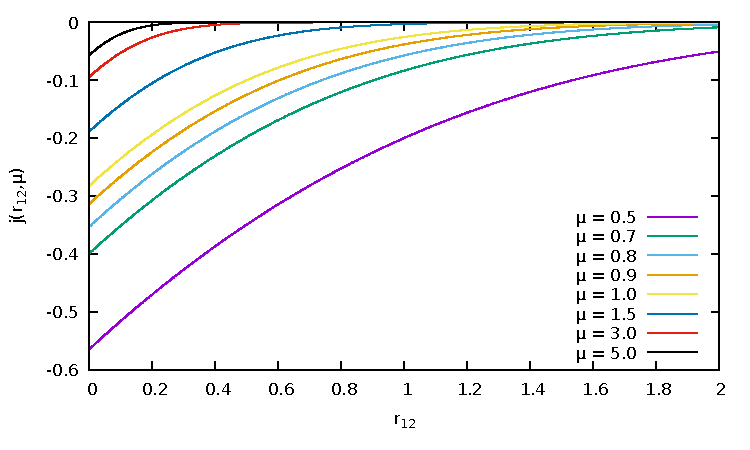
\includegraphics[width=0.45\linewidth]{small_mu_j.pdf}
        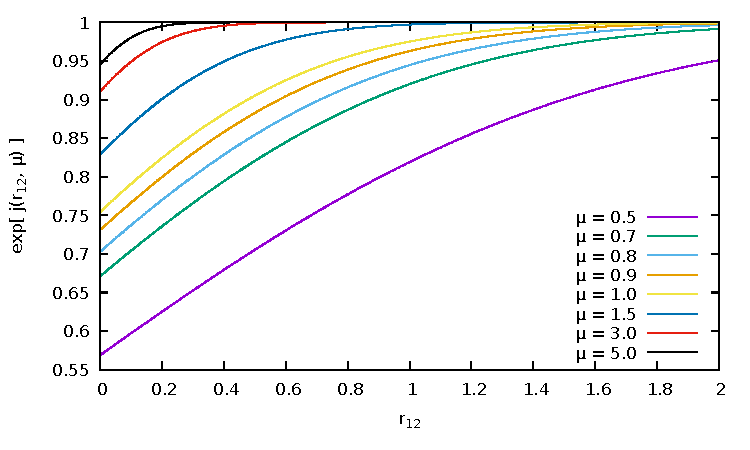
\includegraphics[width=0.45\linewidth]{small_mu_exp_j.pdf}\\
        \caption{Shape of $j(r_{12};\mu)$ (up) and of $\mathcal{J}(r_{12};\mu) = \text{exp}\bigg(j(r_{12};\mu) \bigg) $ (bottom) for different values of $\mu$.}
\end{figure*}
From Figure\ref{fig_j_mu}, one can see that: i) the larger the $\mu$, the more short-range is $j(r_{12};\mu)$, ii) the larger the $\mu$, the closer $j(r_{12};\mu)$ is from 0 and therefore the less impact the correlating factor has on the wave function, iii) the smaller the $\mu$, the deeper is the hole imposed by $\mathcal{J}(r_{12};\mu)$. 


\subsection{Explicit form of  $\tilde{H}[\mu]$ and some of its properties}
\subsubsection{Explicit form of $\tilde{H}[\mu]$ }
Having established the explicit form of $j(r_{12};\mu)$ and some of its properties, one can now 
look at the explicit form of the transcorrelated Hamiltonian obtained with $j(r_{12};\mu)$,  
which, by injecting the form of \eqref{eq:def_j} in Eq.\eqref{eq:ht_phi}, reads 
\begin{equation}
  \begin{aligned}
 \label{eq:exp_ht_mu}
   \tilde{H}[\mu] = & h_c + \frac{\text{erf}(\mu r_{12})}{r_{12}} + \frac{\mu}{\sqrt{\pi}} e^{-\big(\mu r_{12} \big)^2} - \frac{\bigg(1 -     \text{erf}(\mu r_{12}) \bigg)^2}{4} \\
& + \bigg( \text{erf}(\mu r_{12}) - 1\bigg) \deriv{}{r_{12}}{}.
  \end{aligned}
\end{equation}
From Eq.\eqref{eq:exp_ht_mu}, one can define an effective scalar electron-electron interaction $\tilde{\mathcal{W}}_{ee}(r_{12}) $ 
\begin{equation}
 \label{eq:deff_w_new}
 \tilde{\mathcal{W}}_{ee}(r_{12},\mu) = \frac{\text{erf}(\mu r_{12})}{r_{12}} + \frac{\mu}{\sqrt{\pi}} e^{-\big(\mu r_{12} \big)^2} - \frac{\bigg(1 -     \text{erf}(\mu r_{12}) \bigg)^2}{4},
\end{equation}
whose shape is illustrated in Fig\ref{fig_wee_mu}. 
\begin{figure*}
 \label{fig_wee_mu}
        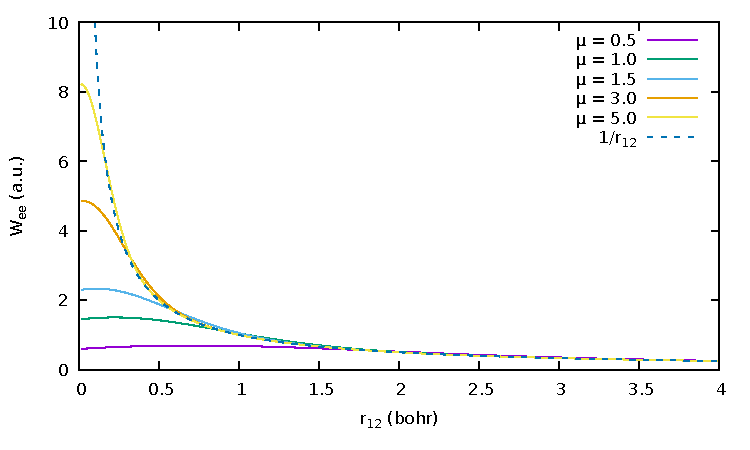
\includegraphics[width=0.45\linewidth]{w_ee.pdf}
        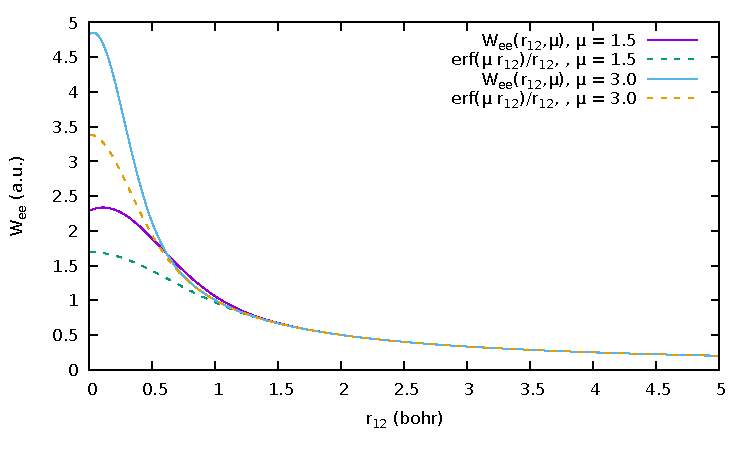
\includegraphics[width=0.45\linewidth]{w_ee_bis.pdf}\\
        \caption{Shape of $\tilde{\mathcal{W}}_{ee}(r_{12},\mu)$ (up) and comparison with $\frac{\text{erf}(\mu r_{12}}{r_{12}}$ (bottom) for different values of $\mu$.}
\end{figure*}
From  Fig.\ref{fig_wee_mu} we can see that the scalar effective potential 
is non divergent, increases when $\mu$ increases and globally resembles the long-range interaction used in RS-DFT at large $r_{12}$. 
Nevertheless, as observed from Fig.\ref{fig_wee_mu}, it is significantly different 
from the long-range interaction at small $r_{12}$, 
and it is not monotonic as it can be even slightly attractive for small values of $\mu$. 
This difference with respect to the long-range interaction can be understood as the equation obtained to derive the Jastrow factor only takes into account the first-order derivative of $j(r_{12},\mu)$ (see Eqs.\eqref{def_j_00} and \eqref{def_j_0}). 
If one desires to impose that $\tilde{\mathcal{W}}_{ee}(r_{12},\mu) = \frac{\text{erf}(\mu r_{12})}{r_{12}}$, one would have to solve the non-linear differential equation 
\begin{equation}
 2 \deriv{j(r_{12})}{r_{12}}{} + r_{12} \bigg( \deriv{j(r_{12})}{r_{12}}{2} + \bigg[ \deriv{j(r_{12})}{r_{12}}{} \bigg]^2\bigg) = 1 - \text{erf}(\mu r_{12}), 
\end{equation}
whose solution is unknown to the best of the author knowledge. 
\subsubsection{Variation of $\tilde{H}[\mu]$ with $\mu$}
\label{sec:h_mu_lim}
Coming now to the limits of $\tilde{H}[\mu]$ when $\mu \rightarrow \infty$, one expects that as
\begin{equation}
 \label{eq:lim_mu_0}
 \lim_{\mu  \rightarrow \infty }j(\mu,r_{12}) = 0, 
\end{equation}
one recovers the usual Hamiltonian in that limit
\begin{equation}
 \label{eq:lim_mu_1}
 \lim_{\mu \rightarrow \infty} \tilde{H}[\mu] = H.
\end{equation}
Nevertheless, in the large $\mu$ limit, one can notice that 
\begin{equation}
 \label{eq:lim_mu_3}
 \lim_{\mu \rightarrow \infty} \tilde{\mathcal{W}}_{ee}(r_{12})  = \frac{1}{r_{12}} + \delta(r_{12}) 
\end{equation}
where $\delta(r_{12})$ is the Dirac distribution, and as the firs-order differential term vanishes in the large $\mu$ limit (see Eq.\eqref{eq:exp_ht_mu}), one could be tempted to write that 
\begin{equation}
 \begin{aligned}
 \label{eq:lim_mu_4}
 \lim_{\mu \rightarrow \infty} \tilde{H}[\mu]& = h_c + \frac{1}{r_{12}} + \delta(r_{12}) \\
                                             & = H + \delta(r_{12})  \\
                                             & \ne H,
 \end{aligned}
\end{equation}
which seems to contradict the intuitive limit of Eq.\eqref{eq:lim_mu_1}. 
Nevertheless, as the right hand side of Eq.\eqref{eq:lim_mu_4} contains a Delta distribution, it must be considered in the sense of distributions an not point wise. 
Therefore, considering $f(\br{}_1,\br{}_2)$, a bounded generic square integrable function in $\R^6$, the equality between $\tilde{H}[\mu]$ and $H$ is, in the sense of distributions, defined by the following equality 
\begin{equation}
 \label{eq:lim_mu_5}
 \begin{aligned}
& \matelem{f}{H}{f} = \lim_{\mu \rightarrow \infty} \matelem{f}{\tilde{H}[\mu]}{f} \\
& \Leftrightarrow H = \tilde{H}[\mu],
 \end{aligned}
\end{equation}
and considering the limit for of $\tilde{H}[\mu]$ (see Eq.\eqref{eq:lim_mu_4}), it implies that 
\begin{equation}
 \label{eq:lim_mu_6}
 \int \text{d}\br{}_1 \text{d}\br{}_2 f(\br{}_1,\br{}_2) \delta(r_{12}) = 0.
\end{equation}
To intuitively show Eq.\eqref{eq:lim_mu_6}, one can perform a series of change of variable $(\br{}_1,\br{}_2)\rightarrow (\br{}_{12},\frac{1}{2}(\br{}_1 + \br{}_2))$ and then use the spherical coordinates for $\br{}_{12}$ and show that 
\begin{equation}
 \int \text{d}\br{}_1 \text{d}\br{}_2 f(\br{}_1,\br{}_2) \delta(r_{12}) = \int \text{d}r{}_{12}  \tilde{f}(r_{12}) \delta(r_{12}) r_{12}^2 
\end{equation}
where $\tilde{f}(x)$ is the function $f(\br{}_1,\br{}_2)$ integrated over $(\br{}_1,\br{}_2)$ with the constraint that 
$|\br{}_1-\br{}_2| = x$. 
As the $f(\br{}_1,\br{}_2)$ remain finite for all $(\br{}_1,\br{}_2)$, the function $\tilde{f}(x)$ 
do not diverge faster than $\frac{1}{x}$ when $x\rightarrow 0$ and therefore one obtains that 
\begin{equation}
 \int \text{d}r{}_{12}  \tilde{f}(r_{12}) \delta(r_{12}) r_{12}^2 = 0,
\end{equation}
and therefore Eq.\eqref{eq:lim_mu_6} which implies Eq.\eqref{eq:lim_mu_1}. 

In the $\mu \rightarrow 0$ limit, the transcorrelated Hamiltonian $\tilde{H}[\mu]$ becomes simply 
\begin{equation}
 \lim_{\mu \rightarrow 0} \tilde{H}[\mu] = h_c - \frac{1}{4} - \partial{}{r_{12}}{}, 
\end{equation}
which means that all scalar electron-electron interaction have been replaced by a differential operator. 

At intermediate values of $\mu$, the scalar potential $\tilde{\mathcal{W}}_{ee}(r_{12},\mu) $ is non divergent but can be either repulsive or attractive at small $r_{12}$. One can therefore notice the diversity of physical content of $\tilde{H}[\mu]$ as a function of a unique parameter, $\mu$. 
Nevertheless, due to the property of the similarity transformation, in the limit of a complete basis set, the eigenvalues of $\tilde{H}[\mu]$, whatever the value of $\mu$ chosen, coincide with that of the physical Hamiltonian. An important point then is the convergence with respect to the basis set of the family of $\tilde{H}[\mu]$ for different values of $\mu$.  

\section{Detailed numerical study of $\tilde{H}[\mu]$ in the case of he He atom}
The first part of our study concerns the convergence of the eigenvalues of $\tilde{H}[\mu]$ with respect to the basis set, and more precisely the dependence on $\mu$ of such convergence. 

Considering a given basis set $\basis$ and the corresponding projector $P_\basis$, one can define the transcorrelated Hamiltonian projected on $\basis$ by
\begin{equation}
 \tilde{H}[\mu]^{\basis} = P_\basis \tilde{H}[\mu] P_\basis,
\end{equation}
and its eigenvalues $E_i^{\basis}[\mu]$ and right eigenvectors $\phiimub$ satisfy 
\begin{equation}
 \tilde{H}[\mu]^{\basis} \ket{\phimub} = E_i^{\basis}[\mu] \ket{\phiimub}. 
\end{equation}
As long as the basis set $\basis$ is incomplete, because of its non hermitian nature, $\tilde{H}[\mu]^{\basis}$ looses the variational principle and therefore its eigenvalues have no reasons to be bounded from below.  

As pointed in section \ref{sec:h_mu_lim}, by varying $\mu$ one can go from a relatively usual repulsive Hamiltonian at large $\mu$ (even though it is non hermitian an non divergent), passing by an almost attractive Hamiltonian and even to a purely attractive Hamiltonian. 
As pointed in section \ref{sec:h_mu_lim}, even though $\tilde{H}[\mu]$ is still non hermitian as long as $\mu < \infty$, by varying $\mu$ one can change the nature of the electron-electron interaction in $\tilde{\mathcal{W}}_{ee}(r_{12},\mu)$ from a repulsive and non divergent interaction at large $\mu$ (an non divergent), passing by an almost attractive Hamiltonian and even to a purely attractive Hamiltonian. 
Considering such variation of $\tilde{H}[\mu]$ when varying $\mu$,  
its projection into a basis set $\tilde{H}[\mu]^{\basis}$ will behave differently as a function of $\mu$ 
and so will the right eigenvectors $\ket{\phiimub}$ and the corresponding eigenvalues $E_i^{\basis}[\mu]$. 
Therefore, we would like to study the behaviour of $\ket{\phiimub}$ and $E_i^{\basis}[\mu]$ as a function of both $\basis$ and $\mu$ to see whether the use of the new form of Jastrow factor $j(r_{12},\mu)$ can improve the convergence toward the exact energies  and eigenvectors. 
\subsection{$\mu$ dependence of the convergence of the ground state eigenvalue with respect to the basis set }
\subsubsection{Computational details}
We implemented all integrals needed for the computation of the matrix elements of $\tilde{H}[\mu]$ on a usual gaussian orbital basis set (see annexes for more details) together with the modification of the Slater rules due to the presence of the non hermitian term in $\tilde{H}[\mu]$. 
All implementation was done as a plugin of the program quantum package\cite{QP2}. 
We use the RHF molecular orbitals to build all matrix elements of $\tilde{H}[\mu]$, and then we solve the two-body problem giving full flexibility to $\Phi_\mu$ (\textit{i.e.} $\Phi_\mu$ is expressed as a linear combination of all possible Slater determinants within a given basis set $\basis$) with a non hermitian eigensolver to obtain both right and left eigenvectors. 
%The study was performed using the augmented Dunning basis aug-cc-pVXZ (X=D,T,Q,5), hereafter referred as AVXZ. 

\subsubsection{Numerical results: ground state energies}
\label{sec:total_e}
We report in Table \ref{table_conv_e_mu} the ground state eigenvalue $E_0^\mu$ of $\tilde{H}[\mu]$ in the AVXZ basis sets (X=D,T,Q,5) for different values of $\mu$, and we report in Figure \ref{fig_conv_e_mu} the graphical representation of such data. 
Several observations can be done from these data. First, because of the loose of the variational principle, $E_0^{\mu}$ can take values below the exact non relativistic energy, and the smaller the $\mu$, the more pronounced is such effect. 
Nevertheless, one can also observe that, for each $\mu$, the error with respect to the reference energy gets smaller  
when enlarging the basis set. Also, qualitatively, one can observe that there are two regimes of $\mu$: $\mu \in[0.05,0.7]$ where the $E_0^\mu$ is always below $E_0$ and $\mu\ge 0.7$ where $E_0^\mu$ converges from above, as if the variational principle still applied. 
As $\mu$ increases, the difference between $E_0^\mu$ and $E_0^\text{FCI}$ in a given basis set diminishes, 
which is expected as in the $\mu \rightarrow \infty$ limit, one obtains that  $\tilde{H}[\mu] \rightarrow H$. 

Coming now to the speed of convergence of $E_0^\mu$ with respect to the basis set, it is always faster than that of $E_0^\text{FCI}$ as long as $\mu \ge 0.2$. 
To quantify better such observations, one can identify the basis set from which the error with respect to the exact non relativistic energy is smaller, in absolute value, than 1mH. 
For $0.3\ge\mu\ge0.4$ one can see that the error with respect to $E_0$ is never larger, in absolute value, than 1mH whatever the basis set used, which represents a strong improvement with respect to the FCI. For $0.5\ge \mu \ge 1.0$ the 1mH error threshold is reached at the aug-cc-pVTZ level and the accuracy are comparable to the FCI in the aug-cc-pV5Z basis set. For $1.6\ge \mu \ge 3.0$, such accuracy is reached at the aug-cc-pVQZ level, whenever such accuracy is reached at the aug-cc-pV5Z level using the regular FCI Hamiltonian. 
Therefore one can conclude that the use of the Jastrow factor $j(r_{12};\mu)$ in the transcorrelated framework can strongly improve the speed of convergence of the total energy of the helium atom with a quite wide range of values of $\mu$ ranging from $\mu=0.2$ to $\mu=1.6$. 
\begin{figure*}
 \label{fig_conv_e_mu}
        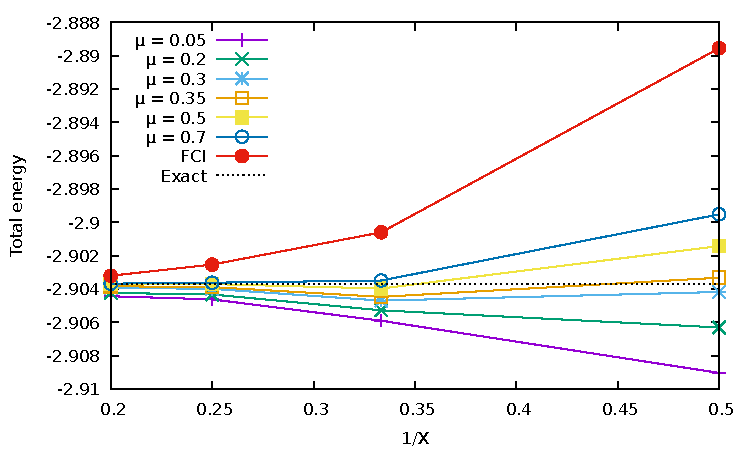
\includegraphics[width=0.45\linewidth]{E_conv_basis_small_mu.pdf}
        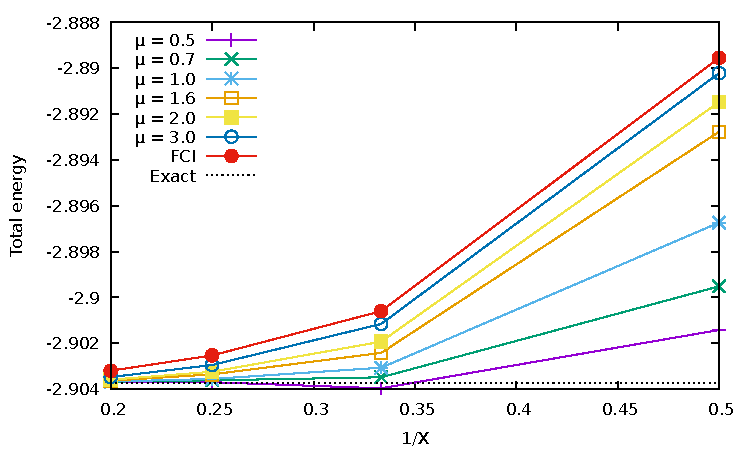
\includegraphics[width=0.45\linewidth]{E_conv_basis_large_mu.pdf}\\
        \caption{Convergence of the ground state eigenvalue of $\tilde{H}[\mu]$ with respect to the AVXZ basis set series (X=D,T,Q,5) for different values of $\mu$.}
\end{figure*}

\begin{table*}
\label{table_conv_e_mu}
\caption{Ground state eigenvalue (in Hartree) of $\tilde{H}[\mu]$ for the He atom with the AVXZ (X=D,T,Q,5) basis sets for different values of $\mu$, and error (in mH) with respect to the exact non relativistic energy.}
\begin{ruledtabular}
\begin{tabular}{llllllllllll}
 Basis/$\mu$&0.05                 & 0.2                   & 0.3                   & 0.35                  & 0.5                  & 0.7                   \\
\hline
 AVDZ       &  -2.909031 (-5.31)  &    -2.906309 (-2.58)  &    -2.904172 (-0.45)  &    -2.903317 (0.41)   &    -2.901420 (2.3)   &    -2.899516 (4.21)   \\
 AVTZ       &  -2.905898 (-2.17)  &    -2.905278 (-1.55)  &    -2.904691 (-0.97)  &    -2.904468 (-0.74)  &    -2.903969 (-0.24) &    -2.903488 (0.24)   \\
 AVQZ       &  -2.904621 (-0.9)   &    -2.904325 (-0.6)   &    -2.903986 (-0.26)  &    -2.903879 (-0.15)  &    -2.903702 (0.02)  &    -2.903620 (0.1)     \\
 AV5Z       &  -2.904428 (-0.7)   &    -2.904229 (-0.51)  &    -2.903928 (-0.2)   &    -2.903834 (-0.11)  &    -2.903702 (0.02)  &    -2.903676 (0.05)   \\
\hline
 Basis/$\mu$ & 1.0                  & 1.6                  & 2.0                  & 3.0                  & $\infty$ (FCI)        & Exact NR              \\
\hline
 AVDZ        &    -2.896734 (6.99)  &    -2.892773 (10.95) &    -2.891477 (12.25) &    -2.890212 (13.51) &    -2.889548 (14.18)  & -2.903724             \\
 AVTZ        &    -2.903069 (0.66)  &    -2.902421 (1.3)   &    -2.901932 (1.79)  &    -2.901159 (2.56)  &    -2.900598 (3.13)   &                       \\
 AVQZ        &    -2.903558 (0.17)  &    -2.903359 (0.36)  &    -2.903244 (0.48)  &    -2.902951 (0.77)  &    -2.902534 (1.19)   &                       \\
 AV5Z        &    -2.903675 (0.05)  &    -2.903634 (0.09)  &    -2.903592 (0.13)  &    -2.903479 (0.24)  &    -2.903201 (0.52)   &                       \\
\end{tabular}
\end{ruledtabular}
\end{table*}

\subsection{Study of the ground state eigenvector in real space}
In Sec.\ref{sec:total_e} we shown the strong improvement of the speed of convergence of the total energy for the helium atom, which was effective for a quite large range of $\mu$ starting from $\mu=0.2$ to $\mu=3.0$. 
Nevertheless, one can wonder if this good behavior results from a kind of error cancellation or if there is indeed a deeper mathematical reason for such an improvement of speed of convergence. 
To answer that question, we investigate some properties of the ground state eigenvectors of different types of Hamiltonians in real space. 

Theoretically if, for a given value of $\mu$, $\tilde{H}[\mu]$ is perfectly well represented in a given basis set $\mathcal{B}$ (\textit{i.e.} $\tilde{H}[\mu]^{\basis} = H$), then all its eigenvalues coincide with that of the exact Hamiltonian (\textit{i.e.} developed in a complete basis set). If one focusses now on the exact ground state eigenvector $\phimu$ of $\tilde{H}[\mu]$, it is directly related to the exact ground state wave function $\psiex$ by the Jastrow factor $j(r_{12},\mu)$ through 
\begin{equation}
 \psiex(\br{}_1,\br{}_2) =  \frac{1}{\sqrt{\mathcal{N}^{\mu}}} e^{j(r_{12},\mu)} \phimu(\br{}_1,\br{}_2), 
\end{equation}
where the normalization factor $\mathcal{N}^{\mu}$ is simply 
\begin{equation}
  \mathcal{N}^{\mu} = \matelem{\phimu}{e^{2 j(r_{12},\mu)}}{\phimu}.
\end{equation}
Therefore, the right eigenvector $\phimub$ of $\tilde{H}[\mu]^{\basis}$ can be used to estimate the exact ground state wave function $\psiex$ through 
\begin{equation}
 \psimub(\br{}_1,\br{}_2) = \frac{1}{\sqrt{\mathcal{N}_{\basis}^{\mu}}}e^{j(r_{12},\mu)}\phimub(\br{}_1,\br{}_2)
\end{equation}
where the normalization factor $\mathcal{N}_{\basis}^{\mu}$ is simply
\begin{equation}
  \mathcal{N}_{\basis}^{\mu} = \matelem{\phimub}{e^{2 j(r_{12},\mu)}}{\phimub}.
\end{equation}
Then, the quality of a given basis set $\basis$ for a given $\mu$ can be also observed from the vicinity between $\psimub(\br{}_1,\br{}_2)$ and the exact wave function $\psiex(\br{}_1,\br{}_2)$. 
For this study, we approximate the exact ground state wave function $\psiex(\br{}_1,\br{}_2)$ of the helium atom by the wave function developed by Umrigar \textit{et. al.}\cite{UmrGon-PRA-94} which contains explicitly the $r_{12}$ coordinate and which provides a total energy accurate up to twelve digits.  
We plotted a cutting of $\psiex(\br{}_1,\br{}_2)$ and  $\psimub(\br{}_1,\br{}_2) $ with different basis sets and values of $\mu$. The cutting used is the following: we set two electrons on a circle of radius $r=0.5$ a.u. from the nucleus and look at the wave functions as a function of the angle $\theta_{12}$ between the electrons. 

We report in Figs \ref{fig:mu_0.3_dz_3} and \ref{fig:mu_1.0_dz_3} the plot of the right eigenvector $\phimub(\br{}_1,\br{}_2)$, estimated exact wave function $\psimub(\br{}_1,\br{}_2)$ for $\mu=0.3$ and $\mu=1.0$ (respectively) and compared to the exact wave function $\psiex(\br{}_1,\br{}_2)$ and FCI wave function for $r=0.5\,a.u.$. 
\begin{figure*}
 \label{fig:mu_0.3_dz_3}
        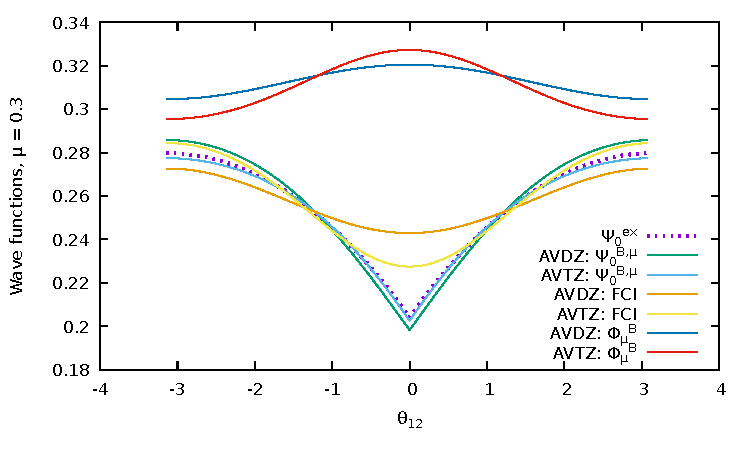
\includegraphics[width=0.45\linewidth]{plots/He//He_mu_0_3_cusp_avdz_avtz_3.pdf}
        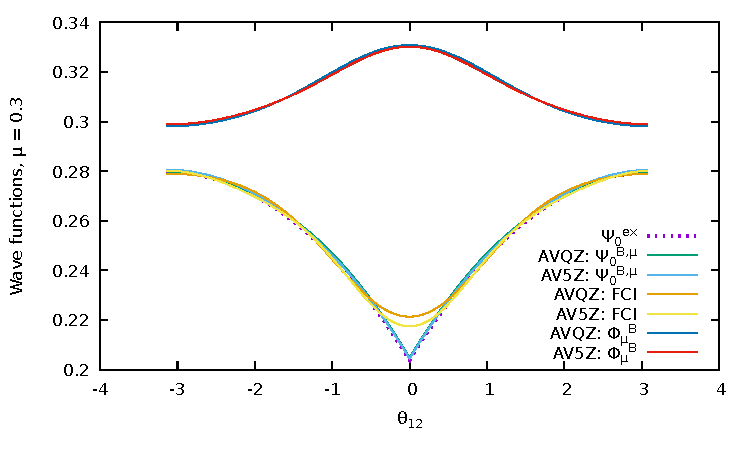
\includegraphics[width=0.45\linewidth]{plots/He/He_mu_0_3_cusp_avqz_av5z_3.pdf}\\
        \caption{
        Helium atom, radius $r=0.5$ a.u.: approximation of the exact wave function $\psimub(\br{}_1,\br{}_2)$ and right eigenvector $\phimub(\br{}_1,\br{}_2)$ for $\mu=0.3$ in the AVDZ and AVTZ basis sets (left) and AVQZ and AV5Z (right). Comparison with the FCI wave function in the same basis sets and the estimated exact wave function $\psiex(\br{}_1,\br{}_2)$.  }
\end{figure*}

\begin{figure*}
 \label{fig:mu_1.0_dz_3}
        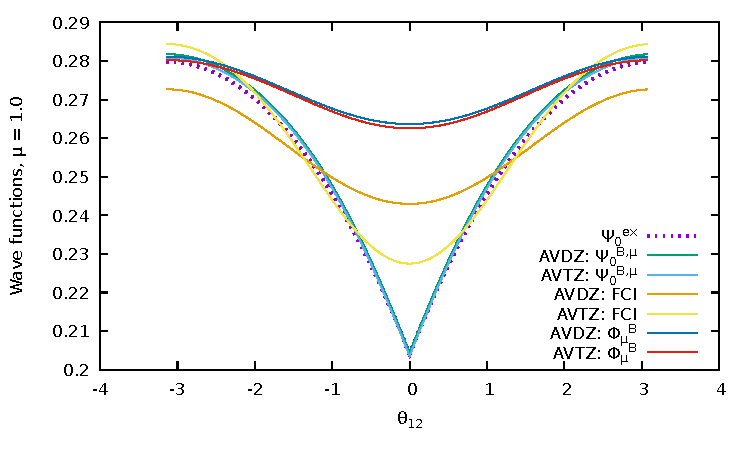
\includegraphics[width=0.45\linewidth]{plots/He/He_mu_1_0_cusp_avdz_avtz_3.pdf}
        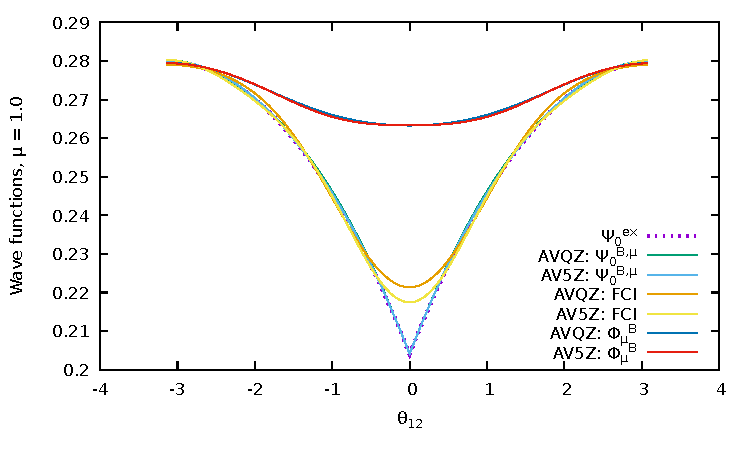
\includegraphics[width=0.45\linewidth]{plots/He/He_mu_1_0_cusp_avqz_av5z_3.pdf}\\
        \caption{
        Helium atom, radius $r=0.5$ a.u.: approximation of the exact wave function $\psimub(\br{}_1,\br{}_2)$ and right eigenvector $\phimub(\br{}_1,\br{}_2)$ for $\mu=1.0$ in the AVDZ and AVTZ basis sets (left) and AVQZ and AV5Z (right). Comparison with the FCI wave function in the same basis sets and the estimated exact wave function $\psiex(\br{}_1,\br{}_2)$.  }
\end{figure*}


From these figure, one can notice that: 
i) the right eigenvector $\phimub(\br{}_1,\br{}_2)$ converges faster than the FCI wave function with respect to the basis set, 
ii) that for $\mu=0.3$ the wave function $\phimub(\br{}_1,\br{}_2)$ present a maximum at $r_{12}=0$, whereas for $\mu=1.0$ and the FCI wave function it has a minimum, 
iii) the wave function $\phimub(\br{}_1,\br{}_2)$ is always larger that the FCI one when $r_{12}\approx 0$. 
iv) that $\psimub(\br{}_1,\br{}_2)$ provides a remarkably good approximation to $\psiex(\br{}_1,\br{}_2)$ from the AVTZ basis set, 

The understanding of such observations can be provided by the mathematical and physical investigation of the construction of $\tilde{H}[\mu]$. 

i) The shape of the Jastrow factor $j(r_{12};\mu)$ leading to the transcorrelated Hamiltonian is such that as long as $\mu < \infty$, the effective potential $\tilde{\mathcal{W}}_{ee}(r_{12},\mu)$ in $\tilde{H}[\mu]$ is non divergent, and therefore its eigenfunctions do not have to fulfill the cusp condition which leads to a faster convergence with $\basis$. 
Nevertheless, one can also remark that for $\mu > 0.5$, the speed of convergence deteriorates as $\mu$ increases, even though it remains finite. This can be explained by the fact that even if $\tilde{\mathcal{W}}_{ee}(r_{12},\mu)$ remains bounded from above, when $\mu$ is large such operator is poorly represented in a finite basis set. 

ii) The fact that the wave function $\phimub(\br{}_1,\br{}_2)$ presents a maximum at $r_{12}=0$ for $\mu=0.3$ whereas it provides a minimum for $\mu=1.0$ or the FCI wave function can be explained by the shape of the effective potential $\tilde{\mathcal{W}}_{ee}(r_{12},\mu)$: the latter is much more attractive when $r_{12}\approx 0$ for $\mu=0.3$ than for $\mu = 1.0$ (see Fig \ref{fig_wee_compare} for a graphical representation). 

iii) Similarly, as for any $\mu < \infty$ one has that $\tilde{\mathcal{W}}_{ee}(r_{12},\mu) <\frac{1}{r_{12}}$, the value of the eigenvector of $\phimub(\br{}_1,\br{}_2)$ is necessary larger than the FCI wave function at $r_{12}=0$ as in the latter the interaction is more repulsive. This implies that the on-top pair density (\textit{i.e.} the probability of finding two electrons at the same position) is necessary larger for the eigenvectors of $\tilde{H}[\mu]$ than that for the eigenvectors of $H$.

iv) The fact that $\psimub(\br{}_1,\br{}_2)$ provides  such a good approximation of $\psiex(\br{}_1,\br{}_2)$ in real space can be investigate through the prism of the local energy. 
The local energy $E_{\text{loc}}[\psi](\br{}_1,\br{}_2)$ associated to a given wave function $\psi$ is defined as 
\begin{equation}
 E_{\text{loc}}[\psi](\br{}_1,\br{}_2) = \frac{H\psi(\br{}_1,\br{}_2)}{\psi(\br{}_1,\br{}_2)},
\end{equation}
and is such that 
\begin{equation}
 \int \text{d}\br{}_1\,\,\text{d}\br{}_2\,\, E_{\text{loc}}[\psi](\br{}_1,\br{}_2) \big|\psi(\br{}_1,\br{}_2)\big|^2= \matelem{\psi}{H}{\psi}.
\end{equation}
Therefore, one can 
\begin{figure*}
 \label{fig_wee_compare}
        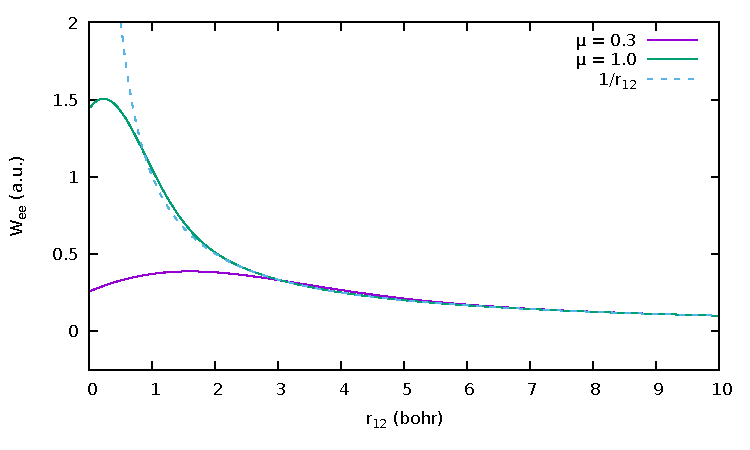
\includegraphics[width=1.00\linewidth]{w_ee_compare.pdf}
        \caption{
        Effective potential $\tilde{\mathcal{W}}_{ee}(r_{12},\mu)$ for $\mu=0.3$ and $\mu=1.0$, compared to the usual $1/r_{12}$ Coulomb interaction.}
\end{figure*}

\section{Study of the helium isoelectronic series}
Having investigated the behaviour of both the eigenvalues and eigenvectors of $\tilde{H}[\mu]$ with $\mu$ and basis set used on the helium atom, we now study the ground state energies of the isoelectronic series of the helium atom H$^{-}$ to Ne$^{8+}$. As seen from the previous study on the helium atom, the quality of the eigenvalues of $\tilde{H}[\mu]$ depend on the value of $\mu$ but there is a quite wide regimes of $\mu$ for which  they  converge significantly faster with the basis set with respect to the usual Hamiltonian. Of course, the 'optimal' range of $\mu$ might depend on the system and we investigate here different approaches to systematically find a reasonable value of $\mu$ and test it on the isoelectronic series of the helium atom. All these systems are weakly correlated, but they cover a quite wide range of densities. 

\subsection{A systematic way to find an optimal value of $\mu$ }
In order to find a systematic way to determine a reasonable value of $\mu$, one must keep in mind the physical meaning of such quantity: it has the unit of an inverse distance, and determines, at leading order, the depth of the hole imposed by the Jastrow factor. 
Therefore, it must have the typical scale of the inverse of correlation effects, which of course strongly depends on the system. In the context of RS-DFT, Toulouse \textit{et. al.}\cite{TouColSav-JCP-05} have investigated different flavour of $\mu$ varying in space through the density of the system in a given point in space. 
More specifically, they introduced (see Eq. (12) of \onlinecite{TouColSav-JCP-05}) a range separation parameter typical for correlation effects in the uniform electron gas (UEG) 
\begin{equation}
 \mursc({\bf r}) =  \frac{2\sqrt{\alpha / \pi}}{\sqrt{r_s({\bf r})}},
\end{equation}
with $\alpha = (9 \pi/4)^{-1/3}$ and $r_s = (4 \pi n/3)^{-1/3}$. 
Such function $\mursc({\bf r})$ depends on the system and on the position in space through the density $n({\bf r})$ of the system at a given point ${\bf r}$. 
Therefore, we propose here to use the average value of $\mursc({\bf r})$ over the Hartree Fock electronic density to define the value of $\mu$ for a specific system in a given basis set:
\begin{equation}
 \murscav = \frac{1}{N_e}\int \text{d}{\bf r} \mursc({\bf r}) n_{\text{HF}}({\bf r}) 
\end{equation}
where $n_{\text{HF}}({\bf r})$ is the HF density and $N_e$ the number of electrons in the system. 
We report in Table \ref{table_conv_e_mu_iso} the convergence with respect to the basis set $\basis$ the error with respect to the exact ground state energies of the isoelectronic series of the helium atom using $\murscav$ as value of $\mu$ in $\tilde{H}[\mu]$. 
As one can observe from  Table \ref{table_conv_e_mu_iso}, the ground state energies of $\tilde{H}[\murscav]$ converge much faster than that of the usual Hamiltonian as the MAD for the ground state energies is of 2.64 mH, 0.48 mH and 0.26 mH in the double-, triple- and quadruple zeta quality basis sets (respectively) whereas it is of 12.16 mH, 4.71 mH and 1.64 mH for the usual Hamiltonian. Also, one can observe that, except for the low density systems such as the H${^-}$ and He species, it converges from below the exact ground state energy. 

In the present context, we propose the derivation of another value of $\mu$ based on the mapping of the on-top pair density of the UEG and a model built with the Jastrow factor defined by \eqref{eq:def_j}. 
For a given point in space ${\bf r}$, we estimate the 
Assuming a single Slater determinant ansatz for a Jastrow Slater wave function with a Jastrow factor defined in \eqref{eq:def_j}, the on-top pair density is 
\begin{equation}
 n_2^\mu({\bf r}) = \frac{1}{2}\big(n({\bf r})\big)^2 e^{-\frac{1}{\sqrt{\pi}\mu}}
\end{equation}
and the exact on-top pair density can be estimated from the UEG through 
\begin{equation}
 n_2^{\text{UEG}}({\bf r}) = \big(n({\bf r})\big)^2g_0(n({\bf r}))
\end{equation}
where $g_0( n)$ is the structure factor of the UEG at a given density $n$. 
Therefore, one can then find the value $\mu$ such that the two on-top pair density coincide
\begin{equation}
 \muueg({\bf r}) = \frac{\text{log}\bigg(2 g_0(n({\bf r}))\bigg) }{\sqrt{\pi}}.
\end{equation}
Therefore one can define an average UEG value of $\mu$.

\begin{table*}
\label{table_conv_e_mu_iso}
\caption{Error (in mH) with respect to the exact non relativistic energies of the ground state eigenvalue of the usual Hamiltonian and $\tilde{H}[\mu]$ for the helium isoelectronic series with Dunning basis sets basis sets for different flavour of $\mu$. For H$^{-}$ and He, the basis sets used are the aug-cc-pVXZ series (X=D,T,Q) and for the Li$^+$-Ne$^{8+}$ series, the cc-pCVXZ (X=D,T,Q) basis sets with core-valence functions were used. The mean absolute deviation (MAD) and mean signed deviation (MSD) are also reported for each basis set and method. }
\begin{ruledtabular}
\begin{tabular}{l|rrr||rrr||rrr|}
             &\multicolumn{3}{c}{H$^-$}      & \multicolumn{3}{c}{He}       & \multicolumn{3}{c}{Li$^+$}    \\
             &   DZ    &  TZ      &   QZ     &  DZ     &   TZ     &  QZ     &   DZ    &   TZ     &  QZ      \\                   
\hline
 FCI         &   3.72  &    1.19  &   0.61   &  14.18  &   3.13   &  1.19   &  10.72  &   3.35   &  1.58    \\      
$\muueg$     &   1.69  &    0.60  &   0.38   &  5.28   &   0.44   &  0.12   &  0.9    &   0.09   & -0.02    \\      
$\murscav$   &   2.30  &    0.67  &   0.39   &  4.87   &   0.37   &  0.12   &  -0.82  &  -0.38   & -0.14    \\      
$\mursclda$  &   2.03  &    0.64  &   0.39   &  5.07   &   0.40   &  0.12   &  0.04   &  -0.12   & -0.08    \\      
\hline
             &\multicolumn{3}{c}{Be$^{2+}$}  & \multicolumn{3}{c}{B$^{3+}$} & \multicolumn{3}{c}{C$^{4+}$}    \\
 FCI         &  11.35  &   3.62   &  1.41    &  11.91  &   4.21   &  1.53   &  12.46  &   4.76   &  1.67    \\  
$\muueg$     &  1.2    &   0.17   & -0.02    &  1.41   &   0.43   &  -0.01  &  1.67   &   0.37   &  0.01    \\  
$\murscav$   &  -1.5   &  -0.53   & -0.17    &  -2.16  &  -0.34   &  -0.22  &  -2.69  &  -0.4    & -0.25    \\  
$\mursclda$  &  -0.08  &  -0.15   & -0.09    &  -0.18  &   0.09   &  -0.11  &  -0.19  &   0.01   &  -0.1    \\  
\hline
             &\multicolumn{3}{c}{N$^{5+}$}   & \multicolumn{3}{c}{O$^{6+}$} & \multicolumn{3}{c}{F$^{7+}$}    \\
 FCI         &  13.1   &   5.71   &  1.79    &  13.84  &   6.47   &  2.02   &  14.68  &   7.06   &  2.25    \\  
$\muueg$     &  2.06   &   0.45   &  0.01    &  2.54   &   0.77   & -0.02   &  3.14   &   1.15   & -0.02    \\  
$\murscav$   &  -2.97  &  -0.64   &  -0.26   & -3.13   &  -0.70   & -0.31   & -3.10   &  -0.54   & -0.36    \\  
$\mursclda$  &  -0.01  &  -0.15   &  -0.09   &  0.27   &  -0.04   & -0.12   &  0.69   &   0.23   & -0.14    \\  
\hline
             &\multicolumn{3}{c}{Ne$^{8+}$}  & \multicolumn{3}{c}{MAD} & \multicolumn{3}{c}{MSD}    \\
 FCI         &  15.66  &   7.61   &  2.36    & 12.16   &    4.71  &    1.64   &  12.16   &   4.71   &    1.64   \\   
$\muueg$     &  3.89   &   1.57   &  0.03    & 4.23    &    1.11  &    0.13   &   4.23   &   1.11   &    0.13   \\   
$\murscav$   &  -2.85  &  -0.28   & -0.35    & 2.64    &    0.48  &    0.26   &  -1.21   &  -0.28   &   -0.16   \\   
$\mursclda$  &  1.26   &   0.57   & -0.1     & 2.38    &    0.60  &    0.07   &   2.38   &   0.60   &    0.05   \\   
\end{tabular}
\end{ruledtabular}
\end{table*}
\section{General formulation of similarity transformed Hamiltonian}
\subsection{General equations for a two-electron system}
According to Eq. (2) of Ref. \onlinecite{CohLuoGutDobTewAla-JCP-19}, the similarity transformed Hamiltonian can be written as 
\begin{equation}
 \label{ht_def_g}
 e^{-\hat{\tau}} \hat{H} e^{\hat{\tau}} = H + \big[ H,\hat{\tau} \big] + \frac{1}{2}\bigg[ \big[H,\hat{\tau}\big],\hat{\tau}\bigg]
\end{equation}
where $\hat{\hat{\tau}} = \sum_{i>j}u(\br{}_i,\br{}_j)$ and $\hat{H} = \sum_i -\frac{1}{2} \nabla^2_i + v(\br{}_i) + \sum_{i>j \frac{1}{r_{ij}}}$. 
This leads to the following similarity transformed Hamiltonian 
\begin{equation}
 \begin{aligned}
 \tilde{H} & = H - \sum_i \bigg( \frac{1}{2} \nabla_i^2 \hat{\tau} + \big(\nabla_i \hat{\tau} \big) + \frac{1}{2} \big(\nabla_i \hat{\tau} \big)  \bigg) \\
           & = H - \sum_{i<j} \hat{K}(\bri{i},\bri{j}) - \sum_{i<j<k} \hat{L}(\bri{i},\bri{j},\bri{k}),
 \end{aligned}
\end{equation}
where the effective two- and three-body operators $\hat{K}(\bri{i},\bri{j})$ and $\hat{L}(\bri{i},\bri{j},\bri{k})$ are defined as
\begin{equation}
 \begin{aligned}
 \label{def_k}
  \hat{K}(\bri{i},\bri{j}) ) = \frac{1}{2} \bigg( &\nabla_i^2 u(\bri{i},\bri{j}) + \nabla_j^2u(\bri{i},\bri{j}) \\
                                               + &\big(\nabla_i u(\bri{i},\bri{j}) \big) ^2 + \big(\nabla_i u(\bri{i},\bri{j}) \big) ^2 \bigg) \\
                                               + &\nabla_i u(\bri{i},\bri{j}) \cdot \nabla_j + \nabla_j u(\bri{i},\bri{j}) \cdot \nabla_i  \\
 \end{aligned}
\end{equation}
\begin{equation}
 \begin{aligned}
 \label{def_k}
  \hat{L}(\bri{i},\bri{j},\bri{k}) ) = & \nabla_i u(\bri{i},\bri{j}) \cdot \nabla_i u(\bri{i},\bri{k}) + \nabla_j u(\bri{j},\bri{i}) \cdot \nabla_j u(\bri{j},\bri{k})  \\
                                     + & \nabla_k u(\bri{k},\bri{i}) \cdot \nabla_k u(\bri{k},\bri{j})
 \end{aligned}
\end{equation}

Of course, only the differential terms do not commute in Eq. \eqref{ht_def_g}. 
Let us compute each terms, beginning with the action of $\big[ H,\hat{\tau} \big]$ on a function $\phi(\br{}_1,\hdots \br{}_N)$.
\begin{equation}
 \label{eq:com1_1}
 \begin{aligned}
 \bigg[ H,\hat{\tau} \bigg]\phi(\br{}_1,\hdots \br{}_N) & = \bigg[ -\frac{1}{2} \sum_i \nabla^2_i, \sum_{j>k} u(\br{}_j,\br{}_k) \bigg] \phi(\br{}_1,\hdots \br{}_N) \\
  & = -\frac{1}{2} \sum_i \nabla^2_i\bigg( \sum_{j>k} u(\br{}_j,\br{}_k) \phi(\br{}_1,\hdots \br{}_N) \bigg) \\
  & +  \frac{1}{2} \sum_{j>k} u(\br{}_j,\br{}_k) \sum_i \nabla^2_i \phi(\br{}_1,\hdots \br{}_N). 
 \end{aligned}
\end{equation}
The first term in the right-hand side of Eq. \eqref{eq:com1_1} is 
\begin{equation}
 \label{eq:com1_2}
 \begin{aligned}
&  -\frac{1}{2} \sum_i \nabla^2_i\bigg( \sum_{j>k} u(\br{}_j,\br{}_k) \phi(\br{}_1,\hdots \br{}_N) \bigg) \\ 
= &-\frac{1}{2}\sum_{j>k} u(\br{}_j,\br{}_k) \sum_i \bigg( \nabla^2_i \phi(\br{}_1,\hdots \br{}_N)\bigg) \\
  &-\frac{1}{2}\phi(\br{}_1,\hdots \br{}_N) \bigg( \sum_i \nabla^2_i \sum_{j>k} u(\br{}_j,\br{}_k) \bigg) \\
  &-\sum_i \bigg(\nabla_i \sum_{j>k}u(\br{}_j,\br{}_k) \bigg) \cdot \bigg( \nabla_i \phi(\br{}_1,\hdots \br{}_N) \bigg).
 \end{aligned}
\end{equation}
Inserting Eq. \eqref{eq:com1_2} in Eq. \eqref{eq:com1_1} leads to cancellation of the terms involving $\nabla^2_i \phi(\br{}_1,\hdots \br{}_N)$
\begin{equation}
 \label{eq:com1_3}
  \begin{aligned}
 \big[ H,\hat{\tau} \big]\phi(\br{}_1,\hdots \br{}_N) & =  \frac{1}{2}\phi(\br{}_1,\hdots \br{}_N) \bigg( \sum_i \nabla^2_i \sum_{j>k} u(\br{}_j,\br{}_k) \bigg) \\
  & -\sum_i \bigg(\nabla_i \sum_{j>k} u(\br{}_j,\br{}_k) \bigg) \cdot \bigg( \nabla_i \phi(\br{}_1,\hdots \br{}_N) \bigg)
 \end{aligned}
\end{equation}
and therefore one can write the first commutator of Eq. \eqref{ht_def_g} as 
\begin{equation}
 \label{eq:com1_4}
 \begin{aligned}
  \big[ H,\hat{\tau} \big] =& -\frac{1}{2} \bigg( \sum_i \nabla^2_i \sum_{j>k} u(\br{}_j,\br{}_k) \bigg) \\
                            & -\sum_i \bigg(\nabla_i \sum_{j>k} u(\br{}_j,\br{}_k) \bigg) \cdot \bigg( \nabla_i  \bigg),
 \end{aligned}
\end{equation}
and as $\nabla_i f(\br{}_j) = \delta_{ij} \nabla_i f(\br{}_i)$ one obtains 
\begin{equation}
 \label{eq:com1_5}
 \begin{aligned}
  \big[ H,\hat{\tau} \big] =& -\frac{1}{2} \bigg( \sum_i \nabla^2_i u(\br{}_i,\br{}_j) + \sum_j \nabla^2_j u(\br{}_i,\br{}_j) ) \bigg) \\
                            & -\sum_i \bigg(\nabla_i u(\br{}_i,\br{}_j)\bigg) \cdot \bigg( \nabla_i  \bigg) \\
                            & -\sum_i \bigg(\nabla_j u(\br{}_i,\br{}_j)\bigg) \cdot \bigg( \nabla_j  \bigg).  
 \end{aligned}
\end{equation}
Then, one has to compute the second-order commutator in Eq. \eqref{ht_def_g}: 
\begin{equation}
 \label{eq:com2_1}
 \begin{aligned}
 & \bigg[ \big[H,\hat{\tau}\big],\hat{\tau}\bigg] \phi(\br{}_1,\hdots \br{}_N) = \\
 & \bigg[ -\frac{1}{2} \bigg( \sum_i \nabla^2_i u(\br{}_i,\br{}_j) + \sum_j \nabla^2_j u(\br{}_i,\br{}_j) ) \bigg), \sum_{j>k} u(\br{}_j,\br{}_k)  \bigg] \phi(\br{}_1,\hdots \br{}_N) \\
+& \bigg[ -\sum_i \bigg(\nabla_i u(\br{}_i,\br{}_j)\bigg) \cdot \bigg( \nabla_i  \bigg), \sum_{j>k} u(\br{}_j,\br{}_k) \bigg] \phi(\br{}_1,\hdots \br{}_N) \\
+& \bigg[ -\sum_i \bigg(\nabla_j u(\br{}_i,\br{}_j)\bigg) \cdot \bigg( \nabla_j  \bigg), \sum_{j>k} u(\br{}_j,\br{}_k) \bigg] \phi(\br{}_1,\hdots \br{}_N). 
 \end{aligned}
\end{equation}
The first term in Eq. \eqref{eq:com2_1} is actually a potential term and therefore it cancels out, then it comes
\begin{equation}
 \label{eq:com2_2}
 \begin{aligned}
  \bigg[ \big[H,\hat{\tau}\big],\hat{\tau}\bigg] = -\sum_i \bigg( \nabla_i u(\br{}_i,\br{}_j) \bigg)^2 - \sum_j \bigg( \nabla_i u(\br{}_i,\br{}_j) \bigg)^2 
 \end{aligned}
\end{equation}
and so the two commutators become
\begin{equation}
 \begin{aligned}
 \label{eq:comtot}
& \big[ H,\hat{\tau} \big] + \frac{1}{2} \bigg[ \big[H,\hat{\tau}\big],\hat{\tau}\bigg] = \\
   &\sum_{i>j} -\frac{1}{2} \bigg( \nabla^2_i u(\br{}_i,\br{}_j) +  \nabla^2_j u(\br{}_i,\br{}_j) 
    + \bigg( \nabla_i u(\br{}_i,\br{}_j) \bigg)^2 + \bigg( \nabla_j u(\br{}_i, \br{}_j) \bigg)^2  \bigg) \\
   & -\bigg(\nabla_i u(\br{}_i,\br{}_j)\bigg) \cdot \bigg( \nabla_i  \bigg) -\bigg(\nabla_j u(\br{}_i,\br{}_j)\bigg) \cdot \bigg( \nabla_j  \bigg). 
 \end{aligned}
\end{equation}

\section{Computations of integrals}
\subsection{$\nabla_i u(\br{}_i,\br{}_j)$}
\begin{equation}
 \nabla_1 u(\br{}_1,\br{}_2) = \deriv{}{x_1}{}u(r_{12}) {\bf e}_{x1} + \deriv{}{y_1}{}u(r_{12}) {\bf e}_{y1} + \deriv{}{z_1}{}u(r_{12}) {\bf e}_{z1},
\end{equation}
and 
\begin{equation}
 \deriv{}{x_1}{}u(r_{12}) = \deriv{}{r_{12}}{}u(r_{12}) \deriv{r_{12}}{x_1}{},
\end{equation}
and as $r_{12} = \sqrt{(x_1 - x_2)^2 + (y_1 - y_2)^2 + (z_1 - z_2)^2} $ one has
\begin{equation}
 \deriv{r_{12}}{x_1}{} = \frac{x_1 - x_2}{r_{12}} = -\deriv{r_{12}}{x_2}{},
\end{equation}
and according to Eq. \eqref{def_j_0}
\begin{equation}
 \deriv{u}{r_{12}}{} = \frac{1 - \text{erf}(\mu r_{12})}{2},
\end{equation}
one obtains 
\begin{equation}
 \label{eq:dx1_u}
 \deriv{}{x_1}{}u(r_{12}) = \frac{1 - \text{erf}(\mu r_{12})}{2 r_{12}} \bigg(x_1 - x_2 \bigg).
\end{equation}
Similarly, 
\begin{equation}
 \label{eq:dx2_u}
 \deriv{}{x_2}{}u(r_{12}) = -\frac{ 1 - \text{erf}(\mu r_{12})}{2 r_{12} } \bigg(x_1 - x_2 \bigg).
\end{equation}
Therefore, 
\begin{equation}
 \label{eq:nabla_u}
 \begin{aligned}
 \nabla_1 u(\br{}_1,\br{}_2) = &\frac{1 - \text{erf}(\mu r_{12})}{2 r_{12}} \\ 
 & \bigg( (x_1 - x_2) {\bf e}_{x1} + (y_1 - y_2) {\bf e}_{y1} + (z_1 - z_2) {\bf e}_{z1}\bigg) \\
 &=  \frac{1 - \text{erf}(\mu r_{12})}{2 r_{12}} \big( \br{}_1 - \br{}_2 \big)
 \end{aligned}
\end{equation}

\subsection{$\bigg(\nabla_i u(\br{}_i,\br{}_j)\bigg)^2$}
According to Eq. \eqref{eq:nabla_u}, one obtains 
\begin{equation}
 \label{eq:nabla_u2_0}
 \begin{aligned}
 \bigg(\nabla_1 u(\br{}_1,\br{}_2)\bigg)^2 & = \bigg( \frac{1 - \text{erf}(\mu r_{12})}{2 r_{12}} \bigg)^2\\
 & \bigg( (x_1 - x_2)^2 + (y_1 - y_2)^2 + (z_1 - z_2)^2 \bigg) \\
                                           &  \frac{\bigg(1 - \text{erf}(\mu r_{12}) \bigg)^2}{4 \big(r_{12}\big)^2} \times \big(r_{12}\big)^2 \\
                                           & = \frac{\bigg(1 - \text{erf}(\mu r_{12}) \bigg)^2}{4}
 \end{aligned}
\end{equation}
and therefore 
\begin{equation}
 \label{eq:nabla_u2}
 \bigg(\nabla_1 u(\br{}_1,\br{}_2)\bigg)^2  + \bigg(\nabla_2 u(\br{}_1,\br{}_2)\bigg)^2 = 2 \times \frac{\bigg(1 - \text{erf}(\mu r_{12}) \bigg)^2}{4}
\end{equation}

\subsection{$\nabla_i u(\br{}_i,\br{}_j) \cdot \bigg( \nabla_i   \bigg)$}
According to Eq. \eqref{eq:nabla_u}, one obtains 
Therefore, 
\begin{equation}
 \begin{aligned}
 \nabla_1 u(\br{}_1,\br{}_2) \cdot \nabla_1  = &\frac{1 - \text{erf}(\mu r_{12})}{2 r_{12}} \\ 
                                          &\bigg( (x_1 - x_2) \deriv{}{x_1}{} + (y_1 - y_2) \deriv{}{y_1}{} + (z_1 - z_2) \deriv{}{z_1}{}\bigg).
 \end{aligned}
\end{equation}
And noticing the minus sign coming from the derivative in $\br{}_2$, the total operator can be written as 
\begin{equation}
 \begin{aligned}
& \nabla_1 u(\br{}_1,\br{}_2) \cdot \nabla_1 + \nabla_2 u(\br{}_1,\br{}_2) \cdot \nabla_2 = \frac{1 - \text{erf}(\mu r_{12})}{2 r_{12}} \\
& \bigg( (x_1 - x_2) \big( \deriv{}{x_1}{} - \deriv{}{x_2}{} \big) +
         (y_1 - y_2) \big( \deriv{}{y_1}{} - \deriv{}{y_2}{} \big) +
         (z_1 - z_2) \big( \deriv{}{z_1}{} - \deriv{}{z_2}{} \big)\bigg),
 \end{aligned}
\end{equation}
but as 
\begin{equation}
 \deriv{}{r_{12}^x}{} = \frac{1}{2} \bigg( \deriv{}{x_1}{} - \deriv{}{x_2}{} \bigg),
\end{equation}
one can rewrite as 
\begin{equation}
 \begin{aligned}
 \label{eq:nabla_i_nabla0}
& \nabla_1 u(\br{}_1,\br{}_2) \cdot \nabla_1 + \nabla_2 u(\br{}_1,\br{}_2) \cdot \nabla_2 = \frac{1 - \text{erf}(\mu r_{12})}{r_{12}} \big( \br{}_1 - \br{}_2 \big) \cdot \nabla_{\br{}_{12}}.
 \end{aligned}
\end{equation}
Then, introducing ${\bf e}_u= \frac{\br{}_1 - \br{}_2}{r_{12}}$, can notice that 
\begin{equation}
 \nabla_{\br{}_{12}} = \deriv{}{r_{12}}{} {\bf e}_u + \frac{1}{r_{12}} \deriv{}{\theta}{} {\bf e}_{\theta} + \frac{1}{r_{12} \sin(\theta)} \deriv{}{\phi}{} {\bf e}_\phi,
\end{equation}
and as $\br{}_1 - \br{}_2 = r_{12} {\bf e}_u$ one obtains
\begin{equation}
 \big( \br{}_1 - \br{}_2 \big) \cdot \nabla_{\br{}_{12}} = r_{12} \deriv{}{r_{12}}{},
\end{equation}
and therefore 
\begin{equation}
 \begin{aligned}
 \label{eq:nabla_i_nabla1}
& \nabla_1 u(\br{}_1,\br{}_2) \cdot \nabla_1 + \nabla_2 u(\br{}_1,\br{}_2) \cdot \nabla_2 = & \frac{1 - \text{erf}(\mu r_{12})}{r_{12}} r_{12} \deriv{}{r_{12}}{} \\
 = & \bigg( 1 - \text{erf}(\mu r_{12})\bigg) \deriv{}{r_{12}}{}. 
 \end{aligned}
\end{equation}


\subsection{$\nabla^2_i u(\br{}_i,\br{}_j)$}
\begin{equation}
 \begin{aligned}
 &\nabla^2_1 u(\br{}_1,\br{}_2) =  \deriv{}{x_{1}}{2}  u(\br{}_1,\br{}_2) + \deriv{}{y_{1}}{2}  u(\br{}_1,\br{}_2) + \deriv{}{z_{1}}{2}  u(\br{}_1,\br{}_2) \\
                                 = & \deriv{}{x_{1}}{}\bigg( \deriv{}{x_{1}}{}u(\br{}_1,\br{}_2) \bigg)  + 
                                   \deriv{}{y_{1}}{}\bigg( \deriv{}{y_{1}}{}u(\br{}_1,\br{}_2) \bigg)  + 
                                   \deriv{}{z_{1}}{}\bigg( \deriv{}{z_{1}}{}u(\br{}_1,\br{}_2) \bigg). 
 \end{aligned}
\end{equation}
But according to Eq. \eqref{eq:dx1_u}, one obtains 
\begin{equation}
 \begin{aligned}
 \label{eq:d2_x1_0}
& \deriv{}{x_{1}}{2}  u(\br{}_1,\br{}_2) = \deriv{}{x_{1}}{}\bigg(\frac{1 - \text{erf}(\mu r_{12})}{2 r_{12}} \big(x_1 - x_2 \big) \bigg) \\
& = \bigg( \deriv{}{x_1}{} \frac{1 - \text{erf}(\mu r_{12})}{2 r_{12}}\bigg) (x_1 - x_2 ) +  \frac{1 - \text{erf}(\mu r_{12})}{2 r_{12}}.
 \end{aligned}
\end{equation}
Similarly, according to Eq. \eqref{eq:dx2_u} one obtains for the second order derivative in $x_2$
\begin{equation}
 \begin{aligned}
 \label{eq:d2_x2_0}
& \deriv{}{x_{2}}{2}  u(\br{}_1,\br{}_2) = \deriv{}{x_{2}}{}\bigg(\frac{\text{erf}(\mu r_{12}) - 1}{2 r_{12}} \big(x_1 - x_2 \big) \bigg) \\
& = \bigg( \deriv{}{x_2}{} \frac{\text{erf}(\mu r_{12}) -1 }{2 r_{12}}\bigg) (x_1 - x_2 ) -  \frac{\text{erf}(\mu r_{12}) -1}{2 r_{12}} \\
& = \bigg( \deriv{}{x_2}{} \frac{\text{erf}(\mu r_{12}) -1 }{2 r_{12}}\bigg) (x_1 - x_2 ) +  \frac{ 1 - \text{erf}(\mu r_{12})}{2 r_{12}}. 
 \end{aligned}
\end{equation}
Also
\begin{equation}
 \label{eq:d2_x1_1}
 \begin{aligned}
 \deriv{}{x_1}{} \frac{1 - \text{erf}(\mu r_{12})}{2 r_{12}} = & \deriv{}{r_{12}}{}\bigg( \frac{1 - \text{erf}(\mu r_{12})}{2 r_{12}}\bigg) \deriv{r_{12}}{x_1}{} \\
      = & \frac{x_1 - x_2}{r_{12}} \deriv{}{r_{12}}{} \frac{1 - \text{erf}(\mu r_{12})}{2 r_{12}} 
 \end{aligned}
\end{equation}
and similarly
\begin{equation}
 \label{eq:d2_x2_1}
 \begin{aligned}
 \deriv{}{x_2}{} \frac{\text{erf}(\mu r_{12}) -  1}{2 r_{12}}  = &\deriv{}{r_{12}}{}\bigg( \frac{\text{erf}(\mu r_{12}) - 1}{2 r_{12}}\bigg) \deriv{r_{12}}{x_2}{} \\
              = & (-1) \frac{x_1 - x_2}{r_{12}} (-1)  \deriv{}{r_{12}}{} \frac{1 - \text{erf}(\mu r_{12})}{2 r_{12}} \\
              = & \frac{x_1 - x_2}{r_{12}} \deriv{}{r_{12}}{} \frac{1 - \text{erf}(\mu r_{12})}{2 r_{12}} \\
              = & \deriv{}{x_1}{} \frac{1 - \text{erf}(\mu r_{12})}{2 r_{12}},
 \end{aligned}
\end{equation}
which implies that 
\begin{equation}
  \label{eq:d2_x2_2}
 \deriv{}{x_{2}}{2}  u(\br{}_1,\br{}_2) = \deriv{}{x_{1}}{2}  u(\br{}_1,\br{}_2).
\end{equation}

To continue, as 
\begin{equation}
 \deriv{}{r_{12}}{} \frac{1 - \text{erf}(\mu r_{12})}{2 r_{12}} = -\frac{1}{r_{12}}\bigg(\frac{1 - \text{erf}\big( \mu r_{12} \big)}{2 r_{12}}  + \frac{\mu}{\sqrt{\pi}} e^{-\big(\mu r_{12} \big)^2} \bigg), 
\end{equation}
one obtains 
\begin{equation}
 \label{eq:d2_x1_2}
 \begin{aligned}
 \deriv{}{x_1}{} \frac{1 - \text{erf}(\mu r_{12})}{2 r_{12}} & = \frac{x_1 - x_2}{r_{12}} \deriv{}{r_{12}}{} \frac{1 - \text{erf}(\mu r_{12})}{2 r_{12}} \\
 & =  -\frac{(x_1 - x_2)}{\big( r_{12} \big)^2}\bigg(\frac{1 - \text{erf}\big( \mu r_{12} \big)}{2 r_{12}}  + \frac{\mu}{\sqrt{\pi}} e^{-\big(\mu r_{12} \big)^2} \bigg). 
 \end{aligned}
\end{equation}

Therefore, Eq. \eqref{eq:d2_x1_0} becomes 
\begin{equation}
 \begin{aligned}
 \label{eq:d2_x1_2}
& \deriv{}{x_{1}}{2}  u(\br{}_1,\br{}_2) = \bigg( \deriv{}{x_1}{} \frac{1 - \text{erf}(\mu r_{12})}{2 r_{12}}\bigg) (x_1 - x_2 ) +  \frac{1 - \text{erf}(\mu r_{12})}{2 r_{12}}  \\
& = -\frac{(x_1 - x_2)^2}{\big( r_{12} \big)^2}\bigg(\frac{1 - \text{erf}\big( \mu r_{12} \big)}{2 r_{12}}  + \frac{\mu}{\sqrt{\pi}} e^{-\big(\mu r_{12} \big)^2} \bigg) +  \frac{1 - \text{erf}(\mu r_{12})}{2 r_{12}} \\
& = \frac{1 - \text{erf}(\mu r_{12})}{2 r_{12}} \bigg( 1 - \frac{(x_1 - x_2)^2}{\big( r_{12} \big)^2} \bigg) 
- \frac{(x_1 - x_2)^2}{\big( r_{12} \big)^2}\frac{\mu}{\sqrt{\pi}} e^{-\big(\mu r_{12} \big)^2},
 \end{aligned}
\end{equation}
implying that 
\begin{equation}
 \begin{aligned}
 \label{eq:d2_x1_3}
 \bigg( \deriv{}{x_{1}}{2} + \deriv{}{y_{1}}{2} + \deriv{}{z_{1}}{2} \bigg)  u(\br{}_1,\br{}_2) = \frac{1 - \text{erf}(\mu r_{12})}{r_{12}} - \frac{\mu}{\sqrt{\pi}} e^{-\big(\mu r_{12}\big)^2},
 \end{aligned}
\end{equation}
and therefore 
\begin{equation}
 \begin{aligned}
 \label{eq:lapl_u_final}
 \bigg( \deriv{}{x_{1}}{2} + \deriv{}{x_{2}}{2} \bigg) u(\br{}_1,\br{}_2) = & \frac{1 - \text{erf}(\mu r_{12})}{r_{12}} \bigg( 1 - \frac{(x_1 - x_2)^2}{\big( r_{12} \big)^2} \bigg) \\ 
&- 2 \frac{(x_1 - x_2)^2}{\big( r_{12} \big)^2}\frac{\mu}{\sqrt{\pi}} e^{-\big(\mu r_{12} \big)^2}.
 \end{aligned}
\end{equation}
Therefore, 
\begin{equation}
 \begin{aligned}
 \label{eq:d2_x1_2}
 &\bigg( \deriv{}{x_{1}}{2} + \deriv{}{x_{2}}{2} + \deriv{}{y_{1}}{2} + \deriv{}{y_{2}}{2} + \deriv{}{z_{1}}{2} + \deriv{}{z_{2}}{2} \bigg) u(\br{}_1,\br{}_2) \\ 
 & =\frac{1 - \text{erf}(\mu r_{12})}{r_{12}} \bigg( 3 - \frac{(x_1 - x_2)^2 + (y_1 - y_2)^2 + (z_1 - z_2)^2}{\big( r_{12} \big)^2} \bigg) \\ 
&- 2 \frac{(x_1 - x_2)^2 + (y_1 - y_2)^2 + (z_1 - z_2)^2}{\big( r_{12} \big)^2}\frac{\mu}{\sqrt{\pi}} e^{-\big(\mu r_{12} \big)^2} \\
 & =\frac{1 - \text{erf}(\mu r_{12})}{r_{12}} \bigg( 3 - \frac{\big(r_{12}\big)^2}{\big( r_{12} \big)^2} \bigg) 
- 2 \frac{\big(r_{12}\big)^2}{\big( r_{12} \big)^2}\frac{\mu}{\sqrt{\pi}} e^{-\big(\mu r_{12} \big)^2} \\
 & =\frac{1 - \text{erf}(\mu r_{12})}{r_{12}} \times 2 - 2 \frac{\mu}{\sqrt{\pi}} e^{-\big(\mu r_{12} \big)^2} \\
 & = 2 \times \bigg( \frac{1 - \text{erf}(\mu r_{12})}{r_{12}} - \frac{\mu}{\sqrt{\pi}} e^{-\big(\mu r_{12} \big)^2}  \bigg)
 \end{aligned}
\end{equation}
\subsection{Sum of all terms}
According to Eq. \eqref{eq:comtot}, Eq. \eqref{eq:nabla_i_nabla1}, Eq. \eqref{eq:nabla_u2} and Eq. \eqref{eq:lapl_u_final}, the additional terms arising from the commutators in $\tilde{H}[j]$ are (for a two-electron system) 
\begin{equation}
 \begin{aligned}
 \label{eq:comtot2}
 & \big[ H,\hat{\tau} \big] + \frac{1}{2} \bigg[ \big[H,\hat{\tau}\big],\hat{\tau}\bigg] =  \\
 & -\frac{1}{2} 2 \times \bigg( \frac{1 - \text{erf}(\mu r_{12})}{r_{12}} - \frac{\mu}{\sqrt{\pi}} e^{-\big(\mu r_{12} \big)^2} + \frac{\bigg(1 - \text{erf}(\mu r_{12}) \bigg)^2}{4}  \bigg) \\
   &- \bigg( 1 - \text{erf}(\mu r_{12})\bigg) \deriv{}{r_{12}}{},
 \end{aligned}
\end{equation}
or equivalently
\begin{equation}
 \begin{aligned}
 \label{eq:comtot2}
 & \big[ H,\hat{\tau} \big] + \frac{1}{2} \bigg[ \big[H,\hat{\tau}\big],\hat{\tau}\bigg] =  \\
 & -\frac{1 - \text{erf}(\mu r_{12})}{r_{12}} + \frac{\mu}{\sqrt{\pi}} e^{-\big(\mu r_{12} \big)^2} - \frac{\bigg(1 - \text{erf}(\mu r_{12}) \bigg)^2}{4} \\
   & + \bigg( \text{erf}(\mu r_{12}) - 1\bigg) \deriv{}{r_{12}}{}.
 \end{aligned}
\end{equation}
Therefore, the full similarity transformed Hamiltonian can be written as
\begin{equation}
  \begin{aligned}
   \tilde{H}[j] = & \sum_{i = 1,2} \bigg( -\frac{1}{2} \big(\nabla_i\big)^2 + v(\br{}_i)  \bigg) + \frac{1}{r_{12}} \\
&   -\frac{1 - \text{erf}(\mu r_{12})}{r_{12}} + \frac{\mu}{\sqrt{\pi}} e^{-\big(\mu r_{12} \big)^2} - \frac{\bigg(1 -     \text{erf}(\mu r_{12}) \bigg)^2}{4} \\
& + \bigg( \text{erf}(\mu r_{12}) - 1\bigg) \deriv{}{r_{12}}{}
  \end{aligned}
\end{equation}
or equivalently 
\begin{equation}
  \begin{aligned}
   \tilde{H}[j] = & h_c + \frac{\text{erf}(\mu r_{12})}{r_{12}} + \frac{\mu}{\sqrt{\pi}} e^{-\big(\mu r_{12} \big)^2} - \frac{\bigg(1 -     \text{erf}(\mu r_{12}) \bigg)^2}{4} \\
& + \bigg( \text{erf}(\mu r_{12}) - 1\bigg) \deriv{}{r_{12}}{},
  \end{aligned}
\end{equation}
which corresponds precisely to Eq. \eqref{eq:h_tilde_r12}. 

\section{Numerical computation of integrals}
\subsection{Fit of functions}
\subsubsection{Fit of $1-\text{erf}(x)$}
At some point we would like to fit the following function
\begin{equation}
 g(x) = 1-\text{erf}(x)
\end{equation}
which can be done, for instance by 
\begin{equation}
 h(x,\alpha,\beta,c) = e^{-\alpha x - \beta x^2}
\end{equation}
with $\alpha=1.09529$ and $\beta = 0.756023$. 
So by posing $y=\mu x$, $x=y/\mu$ then
\begin{equation}
 \label{fit_erf}
 \begin{aligned}
  g(x,\mu)  =& 1 - \text{erf}(\mu x) \approx e^{-\alpha \mu x - \beta (\mu x)^2}\\ 
        =& e^{-\alpha \mu x } e^{-\beta \mu^2 x^2} \\
        =& h(x,\alpha \mu, \beta \mu^2).
 \end{aligned}
\end{equation}
Therefore, one can fit $g(x)^2$ as 
\begin{equation}
 \begin{aligned}
 g(x,\mu)^2 = \bigg( 1 - \text{erf}(\mu x) \bigg)^2\\
           &= \bigg( e^{-\alpha \mu x } e^{-\beta \mu^2 x^2}\bigg)^2 \\
           &= e^{-2\alpha  \mu x } e^{-2 \beta \mu^2 x^2} \\
           &= h(x,2 \alpha \mu, 2 \beta \mu^2).
 \end{aligned}
\end{equation}

\subsubsection{Fit of $e^{-x}$}
The fit of $1 - \text{erf}(\mu x)$ in Eq. \eqref{fit_erf} involves a Slater function, which is always rather complex to integrate. 
Nevertheless, we can fit a Slater function with Gaussian functions (that is what quantum chemistry is about):
\begin{equation}
 e^{-X} = \sum_{m=1}^{N_s} c_m e^{-\zeta_m X^2}, 
\end{equation}
and, by posing $X=\gamma x$ one can fit any Slater function as
\begin{equation}
 e^{-\gamma x} = \sum_{m=1}^{N_s} c_m e^{-\zeta_m \gamma^2 x^2}. 
\end{equation}
To find the $\{c_m,\zeta_m\}$ parameters, I performed a Hartree Fock calculation on the Hydrogen atom using the $s$ functions of the ANO-RCC basis set which contains 8 gaussians.  

\subsection{Computation of integrals with $\text{exp}(-\alpha r_{12}^2)$}
As essentially all functions of $r_{12}$ involve directly or indirectly (\textit{i.e.} through a fit) gaussian functions, we will have to evaluate such integrals
\begin{equation}
 \begin{aligned}
  \int \text{d}\br{}_1  \text{d}\br{}_2& \big( x_1 - A_x \big)^{a_x}  \big( x_2 - B_x \big)^{b_x} 
                                         \big( y_1 - A_y \big)^{a_y}  \big( y_2 - B_y \big)^{b_y} 
                                         \big( z_1 - A_z \big)^{a_z}  \big( z_2 - B_z \big)^{b_z} \\
                                       & \text{exp}(-\alpha \big(\br{}_1 - {\bf A} \big)^2)
                                         \text{exp}(-\beta  \big(\br{}_2 - {\bf B} \big)^2)
                                         \text{exp}(-\delta \big(\br{}_1 - \br{}_2 \big)^2)
 \end{aligned}
\end{equation}
which can be transformed into product of types 
\begin{equation}
 \begin{aligned}
  \int \text{d}x_1 \text{d}x_2 & \big( x_1 - A_x \big)^{a_x} \big( x_2 - B_x \big)^{b_x} \\ 
  & \text{exp}(-\alpha \big(x_1 - A_x \big)^2) \text{exp}(-\alpha \big(x_2 - B_x \big)^2) \text{exp}(-\delta \big(x_1 - x_2 \big)^2)
 \end{aligned}
\end{equation}

\section{New form of jastrow factor}
We want the jastrow factor $j(r_{12})$ to fulfil such equation
\begin{equation}
 - \bigg[ \frac{2}{r_{12}} \deriv{j}{r_{12}}{}  + \deriv{j}{r_{12}}{2} \bigg] + \frac{1}{r_{12}} = \frac{\text{erf}\big( \mu r_{12} \big)}{r_{12}}.
\end{equation}
The solution for such an equation is 
\begin{equation}
 j(r_{12}) = \frac{1}{2}r_{12}\bigg( 1 - \text{erf}(\mu r_{12}) \bigg) - \frac{1}{2\sqrt{\pi} \mu} e^{-\big( \mu r_{12}\big)^2} + \frac{1}{4 r_{12}} \bigg(c_1 - \frac{\text{erf}\big(\mu r_{12} \big)}{\mu^2} \bigg).
\end{equation}
The constant $c_1$ can be found to impose that 
\begin{equation}
 \lim_{r_{12} \rightarrow 0 } j(r_{12}) < \infty,
\end{equation}
which means $c_1 = 0$. Therefore the new jastrow factor is 
\begin{equation}
 j(r_{12}) = \frac{1}{2}r_{12}\bigg( 1 - \text{erf}(\mu r_{12}) \bigg) - \frac{1}{2\sqrt{\pi} \mu} e^{-\big( \mu r_{12}\big)^2}  - \frac{\text{erf}\big(\mu r_{12} \big)}{4 \mu^2 r_{12}}.
\end{equation}

\section{One body term jastrow}
\subsection{The case of the Hydrogen atom}
We want to find a Jastrow factor which will take care of the nuclear-electron cusp condition, and we will begin by the Hydrogen atom.  

Let us write the Hamiltonian of the hydrogenoid atom in the radial coordinate for the $l=0$ sector 
\begin{equation}
 H = -\frac{1}{2} \big( \deriv{}{r}{2} + \frac{2}{r} \deriv{}{r}{}\big) - \frac{Z}{r}.
\end{equation}
To do so, we have to compute the kinetic part acting on the Jastrow factor acting on a function depending only on the radial coordinate $\phi( r)$
\begin{equation}
 \label{eq:h_atom_j}
 \begin{aligned}
 & -\frac{1}{2}e^{-j(r)}\big(\deriv{}{r}{2} + \frac{2}{r} \deriv{}{r}{} \big) e^{j(r)}\phi(r)  = \\
 & -\frac{1}{2}\big( \deriv{}{r}{2} + \frac{2}{r} \deriv{}{r}{} \big) \phi(r) \\
 &-\deriv{j(r)}{r}{}\deriv{}{r}{}\phi(r) \\
 &-\frac{1}{r}\deriv{j(r)}{r}{}\phi(r)  - \frac{1}{2}\deriv{j(r)}{r}{2}\phi(r)  -  \frac{1}{2}\bigg(\deriv{j(r)}{r}{} \bigg)^2 \phi(r).
 \end{aligned}
\end{equation}
Therefore the full similarity transformed Hamiltonian $\tilde{H}[j]$ is 
\begin{equation}
 \begin{aligned}
 \label{eq:one_e_0}
 & e^{-j(r)}H\,e^{j(r)} = \\
 & -\frac{1}{2}\big( \deriv{}{r}{2} + \frac{2}{r} \deriv{}{r}{} \big) -\deriv{j(r)}{r}{}\deriv{}{r}{}\\
 &-\frac{1}{r}\bigg(\deriv{j(r)}{r}{} + Z \bigg) \\ 
 & - \frac{1}{2}\deriv{j(r)}{r}{2} -  \frac{1}{2}\bigg(\deriv{j(r)}{r}{} \bigg)^2.
 \end{aligned}
\end{equation}
Similarly to what have been proposed in Section \ref{sec:he_j}, we want to find the Jastrow factor $j(r,\mu,Z)$ such that 
\begin{equation}
 \label{eq:one_e_01}
 -\frac{1}{r}\bigg(\deriv{j(r,\mu,Z)}{r}{} + Z \bigg) = -Z\frac{\text{erf}(\mu r)}{r},
\end{equation}
or equivalently
\begin{equation}
 \label{eq:one_e_1}
 \deriv{}{r}{}j(r,\mu,Z) = Z\bigg( \text{erf}(\mu r) - 1\bigg).
\end{equation}
The Jastrow factor fulfilling Eq. \eqref{eq:one_e_1} is 
\begin{equation}
 \label{eq:one_e_2}
 j(r,\mu,Z) = -Z r \bigg( 1 - \text{erf}\big(\mu r\big) \bigg) + \frac{Z}{\sqrt{\pi}\mu} e^{-\big(\mu r \big)^2}. 
\end{equation}
Now, we can plug $j(r,\mu,Z)$ into Eq. \eqref{eq:one_e_0} in order to compute the explicit form of the similarity transformed Hamiltonian. 
To do so, we use Eq. \eqref{eq:one_e_1}, and also that 
\begin{equation}
 \deriv{}{r}{2}j(r) = \frac{2 \mu Z }{\sqrt{\pi}} e^{-(\mu r)^2}.
\end{equation}
One obtains then the similarity transformed Hamiltonian 
\begin{equation}
 \begin{aligned}
 \tilde{H}[j] = & e^{-j(r)} H e^{j(r)} \\
              = & -\frac{1}{2}\big( \deriv{}{r}{2} + \frac{2}{r} \deriv{}{r}{} \big) - \frac{Z}{r}  \\
                & + Z \bigg( 1 - \text{erf}(\mu r)\bigg) \deriv{}{r}{} \\
                & - Z \frac{\text{erf}(\mu r) - 1}{r} \\
                & -Z \frac{\mu}{\sqrt{\pi}} e^{-(\mu r)^2} \\
                & - \frac{1}{2}Z^2 \bigg( \text{erf}(\mu r) -1 \bigg)^2,
 \end{aligned}
\end{equation}
and one can notice that the $\frac{-Z}{r}$ interaction cancels out to give
\begin{equation}
 \label{eq:one_e_3}
 \begin{aligned}
 \tilde{H}[j] = & e^{-j(r)} H e^{j(r)} \\
              = & -\frac{1}{2}\big( \deriv{}{r}{2} + \frac{2}{r} \deriv{}{r}{} \big)  \\
                & -Z \bigg[ \frac{\mu}{\sqrt{\pi}} e^{-(\mu r)^2} + \frac{\text{erf}(\mu r)}{r} + \frac{1}{2}Z \bigg( \text{erf}(\mu r) -1 \bigg)^2 \bigg] \\
                & + Z \bigg( 1 - \text{erf}(\mu r)\bigg) \deriv{}{r}{}. 
 \end{aligned}
\end{equation}
Therefore, compared to the usual Hamiltonian, the similarity transformed Hamiltonian contains a different local interaction which is clearly non divergent, but also a new short-range differential operator. 

\subsection{General equation}
Now that we know the general form of the one-body Jastrow factor for a one electron system, we can generalize it 
to an $N$-electron system and an $M$ nucleus system by just taking the following form 
\begin{equation}
 e^{\hat{\tau}({\bf r}_1,\hdots , {\bf r}_i,{\bf r}_N)} = e^{-\sum_i^N J({\bf r}_i)} 
\end{equation}
where $J({\bf r}_i)$ has the following form 
\begin{equation}
 J({\bf r}_i) = \sum_{A} j(r_{iA},\mu,Z_A) 
\end{equation}
where $j(r,\mu,Z)$ is given by Eq. \eqref{eq:one_e_2} and $r_{iA} = \big|{\bf r}_i - {\bf R}_A \big|$. 
According to Eq. (2) of Ref. \onlinecite{CohLuoGutDobTewAla-JCP-19}, the equation of the similarity transformed Hamiltonian is similar  
to that of Eq. \eqref{ht_def_g} but with a new form of Jastrow factor. 
Therefore one needs to compute $\big[ H,\hat{\tau} \big]$ and $\frac{1}{2}\bigg[ \big[H,\hat{\tau}\big],\hat{\tau}\bigg]$. 
Let us begin by $\big[ H,\hat{\tau} \big]$, and as before, we apply it to a general function $\phi(\br{}_1,\hdots \br{}_N)$:
\begin{equation}
 \label{eq:one_com1_1}
 \begin{aligned}
 \bigg[ H, \hat{\tau} \bigg]\phi(\br{}_1,\hdots \br{}_N) & = \bigg[ -\frac{1}{2} \sum_i \nabla^2_i, \sum_{j} J(\br{}_j) \bigg]      \phi(\br{}_1,\hdots \br{}_N) \\    
                                                        & = -\frac{1}{2} \sum_i \bigg( \big(\nabla^2_i J({\bf r}_i)\big) + 2\nabla_i J({\bf r}_i) \cdot \nabla_i \phi(\br{}_1,\hdots \br{}_N) \bigg).  
 \end{aligned}
\end{equation}
Therefore, one can write that term as
\begin{equation}
 \label{eq:one_com1_2}
 \begin{aligned}
  \big[ H,\hat{\tau} \big] =& -\frac{1}{2} \bigg( \sum_i \nabla^2_i J(\br{}_i) \bigg) \\
                            & -\sum_i \bigg(\nabla_i J(\br{}_i) \bigg) \cdot \bigg( \nabla_i  \bigg).
 \end{aligned}
\end{equation}
After some math, the second-order commutator is simply 
\begin{equation}
 \bigg[ \big[H,\hat{\tau}\big],\hat{\tau}\bigg] = -\sum_i \nabla_i J({\bf r}_i) \cdot \nabla_i J({\bf r}_i) 
\end{equation}
So eventually, the similarity transformed operator becomes 
\begin{equation}
 \begin{aligned}
& H + \big[ H,\hat{\tau} \big] + \frac{1}{2} \bigg[ \big[H,\hat{\tau}\big],\hat{\tau}\bigg] = \\ & H -\frac{1}{2} \bigg( \sum_i \nabla^2_i J(\br{}_i) \bigg)    
                                                                   -\sum_i \bigg(\nabla_i J(\br{}_i) \bigg) \cdot \bigg( \nabla_i  \bigg)  
                                                                   -\frac{1}{2}\sum_i \nabla_i J({\bf r}_i) \cdot \nabla_i J({\bf r}_i) 
 \end{aligned}
\end{equation}
Therefore, the addition of the jastrow operator does not add extra two-body terms. 
\subsection{Computation of the total operator}
\subsubsection{Computation of $\nabla_i J(\br{}_i)$}
\begin{equation}
 \begin{aligned}
&\nabla_i J(\br{}_i) = \sum_A \nabla_i J(r_{iA},Z_A) \\
                    &= \sum_A \deriv{}{x_i}{} J(r_{iA},Z_A) {\bf e}_{x_i} + \deriv{}{y_i}{} J(r_{iA},Z_A) {\bf e}_{y_i} + \deriv{}{z_i}{} J(r_{iA},Z_A) {\bf e}_{z_i}, 
 \end{aligned}
\end{equation}
and 
\begin{equation}
 \deriv{}{x_i}{}J(r_{iA}) = \deriv{}{r_{iA}}{}J(r_{iA}) \deriv{r_{iA}}{x_i}{},
\end{equation}
and as $r_{iA} = \sqrt{(x_1 - x_A)^2 + (y_1 - y_A)^2 + (z_1 - z_A)^2} $ 
one has                                                              
\begin{equation}
 \deriv{r_{iA}}{x_1}{} = \frac{x_1 - x_A}{r_{iA}}
\end{equation}
and therefore according to Eq. \eqref{eq:one_e_1}, one has 
\begin{equation}
 \deriv{}{x_i}{} J(r_{iA},Z_A) = -\sum_A Z_A \big( x_i - x_A \big) \frac{1 - \text{erf}(\mu r_{iA})}{r_{iA}}.
\end{equation}
\subsubsection{Computation of $\nabla_i J({\bf r}_i) \cdot \nabla_i J({\bf r}_i)$}
The computation of $\nabla_i J({\bf r}_i) \cdot \nabla_i J({\bf r}_i)$ leads to 
\begin{equation}
 \begin{aligned}
  \nabla_i J({\bf r}_i) \cdot \nabla_i J({\bf r}_i) =  \sum_{A,B} Z_B &Z_A \big( x_i - x_A \big) \big( x_i - x_B \big)  \frac{ 1 -\text{erf}(\mu r_{iA})}{r_{iA}} \frac{ 1 - \text{erf}(\mu r_{iB})}{r_{iB}} \\
                                                                      & +  \big( y_i - y_A \big) \big( y_i - y_B \big)  \frac{ 1 -\text{erf}(\mu r_{iA})}{r_{iA}} \frac{ 1 - \text{erf}(\mu r_{iB})}{r_{iB}} \\ 
                                                                      & +  \big( z_i - z_A \big) \big( z_i - z_B \big)  \frac{ 1 -\text{erf}(\mu r_{iA})}{r_{iA}} \frac{ 1 - \text{erf}(\mu r_{iB})}{r_{iB}}.
 \end{aligned}
\end{equation}
The diagonal part of such integrals is simply
\begin{equation}
 \begin{aligned}
 &  \sum_{A} (Z_A)^2 \bigg(\big( x_i - x_A \big)^2 +  \big( y_i - y_A \big)^2 + \big( z_i - z_A \big)^2\bigg) \frac{\bigg(\text{erf}(\mu r_{iA}) - 1\bigg)^2}{\big(r_{iA}\big)^2}\\ 
  = & \sum_{A} (Z_A)^2 \bigg( \text{erf}(\mu r_{iA}) -1 \bigg)^2
 \end{aligned}
\end{equation}


\subsubsection{Computation of $\nabla^2_i J(\br{}_i) $}
We need to compute 
\begin{equation}
 \begin{aligned}
 \deriv{}{x_{i}}{2} J(\br{}_i) & = -\sum_A Z_A \deriv{}{x_i}{} \bigg[(x_i - x_A) \frac{1 - \text{erf}(\mu r)}{r_{iA}} \bigg] \\
                               & = -\sum_A Z_A \bigg[ \frac{1 - \text{erf}(\mu r_{iA})}{r_{iA}} + (x_i - x_A) \deriv{}{x_i}{}\frac{1 - \text{erf}(\mu r_{iA})}{r_{iA}}  \bigg]
 \end{aligned}
\end{equation}
But, one has that
\begin{equation}
 \begin{aligned}
 \deriv{}{x_i}{} \frac{1 - \text{erf}(\mu r_{iA})}{r_{iA}} = - \frac{(x_i - x_A)}{(r_{iA})^2} \bigg( \frac{2 \mu}{\sqrt{\pi}} e^{-(\mu r_{iA})^2} + \frac{1 - \text{erf}(\mu r_{iA})}{r_{iA}}\bigg).
 \end{aligned}
\end{equation}
Therefore, 
\begin{equation}
 \label{eq:lapl_important}
 (x_i - x_A) \deriv{}{x_i}{}\frac{1 - \text{erf}(\mu r_{iA})}{r_{iA}} = - \frac{(x_i - x_A)^2}{(r_{iA})^2} \bigg( \frac{2 \mu}{\sqrt{\pi}} e^{-(\mu r_{iA})^2} + \frac{1 - \text{erf}(\mu r_{iA})}{r_{iA}}\bigg)
\end{equation}.
Therefore, the Laplacian is 
\begin{equation}
 \begin{aligned}
 \label{eq:lapl_interm_1}
&  \deriv{}{x_{i}}{2} J(\br{}_i) + \deriv{}{y_{i}}{2} J(\br{}_i) + \deriv{}{z_{i}}{2} J(\br{}_i) =  - \sum_{A} Z_A \bigg[ 3 \frac{1 - \text{erf}(\mu r_{iA})}{r_{iA}}  \\
 & + (x_i - x_A) \deriv{}{x_i}{}\frac{1 - \text{erf}(\mu r_{iA})}{r_{iA}} \\ 
 & + (y_i - y_A) \deriv{}{y_i}{}\frac{1 - \text{erf}(\mu r_{iA})}{r_{iA}} \\ 
 & + (z_i - z_A) \deriv{}{z_i}{}\frac{1 - \text{erf}(\mu r_{iA})}{r_{iA}}  \bigg]
 \end{aligned}
\end{equation}
But according to Eq. \eqref{eq:lapl_important}, one has that 
\begin{equation}
 \begin{aligned}
 & + (x_i - x_A) \deriv{}{x_i}{}\frac{1 - \text{erf}(\mu r_{iA})}{r_{iA}} \\ 
 & + (y_i - y_A) \deriv{}{y_i}{}\frac{1 - \text{erf}(\mu r_{iA})}{r_{iA}} \\ 
 & + (z_i - z_A) \deriv{}{z_i}{}\frac{1 - \text{erf}(\mu r_{iA})}{r_{iA}}  = \\
 &- \frac{(x_i - x_A)^2 + (y_i - y_A)^2 + (z_i - z_A)^2}{(r_{iA})^2} \bigg( \frac{2 \mu}{\sqrt{\pi}} e^{-(\mu r_{iA})^2} + \frac{1 - \text{erf}(\mu r_{iA})}{r_{iA}}\bigg)
 \end{aligned}
\end{equation}
which is simply 
\begin{equation}
 \begin{aligned}
 \label{eq:lapl_interm_2}
 & + (x_i - x_A) \deriv{}{x_i}{}\frac{1 - \text{erf}(\mu r_{iA})}{r_{iA}} \\ 
 & + (y_i - y_A) \deriv{}{y_i}{}\frac{1 - \text{erf}(\mu r_{iA})}{r_{iA}} \\ 
 & + (z_i - z_A) \deriv{}{z_i}{}\frac{1 - \text{erf}(\mu r_{iA})}{r_{iA}}  = \\
 &- \bigg( \frac{2 \mu}{\sqrt{\pi}} e^{-(\mu r_{iA})^2} + \frac{1 - \text{erf}(\mu r_{iA})}{r_{iA}}\bigg).
 \end{aligned}
\end{equation}
Then, coming back to Eq. \eqref{eq:lapl_interm_1} with Eq. \eqref{eq:lapl_interm_2} one has 
\begin{equation}
 \Delta_i J(\br{}_i) = - \sum_{A}  Z_A \bigg[ 3 \frac{1 - \text{erf}(\mu r_{iA})}{r_{iA}}  - \bigg( \frac{2 \mu}{\sqrt{\pi}} e^{-(\mu r_{iA})^2} + \frac{1 - \text{erf}(\mu r_{iA})}{r_{iA}}\bigg) \bigg]
\end{equation}
which becomes 
\begin{equation}
 \Delta_i J(\br{}_i) = - \sum_{A}  2 \, Z_A  \bigg[ \frac{1 - \text{erf}(\mu r_{iA})}{r_{iA}}  - \frac{\mu}{\sqrt{\pi}} e^{-(\mu r_{iA})^2}  \bigg]
\end{equation}
\subsubsection{Computation of the total operator}
\begin{equation}
 \begin{aligned}
& H + \big[ H,\hat{\tau} \big] + \frac{1}{2} \bigg[ \big[H,\hat{\tau}\big],J\bigg] = \\ & H -\frac{1}{2} \bigg( \sum_i \nabla^2_i J(\br{}_i) \bigg)    
                                                                   -\sum_i \bigg(\nabla_i J(\br{}_i) \bigg) \cdot \bigg( \nabla_i  \bigg)  
                                                                   -\frac{1}{2}\sum_i \nabla_i J({\bf r}_i) \cdot \nabla_i J({\bf r}_i) 
 \end{aligned}
\end{equation}
which becomes
\begin{equation}
 \begin{aligned}
  \tilde{H} = H +&  \sum_i \sum_{A}\, Z_A  \bigg[ \frac{1 - \text{erf}(\mu r_{iA})}{r_{iA}}  - \frac{\mu}{\sqrt{\pi}} e^{-(\mu r_{iA})^2}  \bigg] \\
           &+  \frac{1 - \text{erf}(\mu r_{iA})}{r_{iA}} \bigg[ (x_i - x_A) \deriv{}{x_i}{} + (y_i - y_A) \deriv{}{y_i}{} + (z_i - z_A) \deriv{}{z_i}{}\bigg] \\
           - \frac{1}{2}\sum_{B} Z_B &\bigg[ \big( x_1 - x_A \big) \big( x_1 - x_B \big)  \frac{\text{erf}(\mu r_{iA}) - 1}{r_{iA}} \frac{\text{erf}(\mu r_{iB}) - 1}{r_{iB}} \\
           &+  \big( y_1 - y_A \big) \big( y_1 - y_B \big)  \frac{\text{erf}(\mu r_{iA}) - 1}{r_{iA}} \frac{\text{erf}(\mu r_{iB}) - 1}{r_{iB}} \\ 
           &+  \big( z_1 - z_A \big) \big( z_1 - z_B \big)  \frac{\text{erf}(\mu r_{iA}) - 1}{r_{iA}} \frac{\text{erf}(\mu r_{iB}) - 1}{r_{iB} } \bigg].
 \end{aligned}
\end{equation}
and as $H = \sum_i -\frac{1}{2} \Delta_i - \sum_A \frac{Z_A}{r_{iA}} + \sum_{i>j} \frac{1}{r_{ij}} $ the total interaction becomes 
\begin{equation}
 \label{eq:final_one_e_h}
 \tilde{H} =  \sum_i -\frac{1}{2} \Delta_i + \sum_A Z_A \tilde{v}_A({\bf r}_i)  + \sum_{i>j} \frac{1}{r_{ij}}
\end{equation}
where the new effective potential is 
\begin{equation}
 \label{eq:final_one_e_v}
 \begin{aligned}
  \tilde{v}_A({\bf r}_i) = & -\frac{\text{erf}(\mu r_{iA})}{r_{iA}} - \frac{\mu}{\sqrt{\pi}} e^{-(\mu r_{iA})^2} \\
           &+  \frac{1 - \text{erf}(\mu r_{iA})}{r_{iA}} \bigg[ (x_i - x_A) \deriv{}{x_i}{} + (y_i - y_A) \deriv{}{y_i}{} + (z_i - z_A) \deriv{}{z_i}{}\bigg] \\
           - \frac{1}{2}\sum_{B} Z_B\bigg[& \big( x_i - x_A \big) \big( x_i - x_B \big)  \frac{\text{erf}(\mu r_{iA}) - 1}{r_{iA}} \frac{\text{erf}(\mu r_{iB}) - 1}{r_{iB}} \\
           +&  \big( y_i - y_A \big) \big( y_i - y_B \big)  \frac{\text{erf}(\mu r_{iA}) - 1}{r_{iA}} \frac{\text{erf}(\mu r_{iB}) - 1}{r_{iB}} \\ 
           +&  \big( z_i - z_A \big) \big( z_i - z_B \big)  \frac{\text{erf}(\mu r_{iA}) - 1}{r_{iA}} \frac{\text{erf}(\mu r_{iB}) - 1}{r_{iB}}\bigg].
 \end{aligned}
\end{equation}
\subsubsection{Verification with the Hydrogen atom}
Let us apply the general equations (see Eqs. \eqref{eq:final_one_e_h} and \eqref{eq:final_one_e_v}) to the case of the Hydrogen atom, which is supposed to be in the center of the frame of reference (\textit{i.e.} ${\bf r}_A = \vec{0}$)
\begin{equation}
 \begin{aligned}
  \tilde{v}({\bf r}) = & -\frac{\text{erf}(\mu r)}{r} - \frac{\mu}{\sqrt{\pi}} e^{-(\mu r)^2} \\
           &+  \frac{1 - \text{erf}(\mu r)}{r} \bigg[ x \deriv{}{x}{} + y \deriv{}{y}{} + z \deriv{}{z}{}\bigg] \\
           &- \frac{1}{2}Z \big(x^2 + y^2 + z^2 \big)  \frac{\big(\text{erf}(\mu r) - 1\big)^2}{r^2},
 \end{aligned}
\end{equation}
but as $r^2 = x^2+y^2+z^2$ one obtains that 
\begin{equation}
 - \frac{1}{2}Z \big(x^2 + y^2 + z^2 \big)  \frac{\big(\text{erf}(\mu r) - 1\big)^2}{r^2} = - \frac{1}{2}Z\big(\text{erf}(\mu r) - 1\big)^2
\end{equation}
and also as 
\begin{equation}
 \begin{aligned}
 x \deriv{}{x}{} + y \deriv{}{y}{} + z \deriv{}{z}{} & = {\bf r} \cdot \nabla \\
                                                     & = r \deriv{}{r}{},
 \end{aligned}
\end{equation}
one obtains 
\begin{equation}
           +  \frac{1 - \text{erf}(\mu r)}{r} \bigg[ x \deriv{}{x}{} + y \deriv{}{y}{} + z \deriv{}{z}{}\bigg] = \bigg(1 - \text{erf}(\mu r)\bigg)\deriv{}{r}{},
\end{equation}
and therefore the total potential is 
\begin{equation}
 \begin{aligned}
  \tilde{v}({\bf r}) = & -\frac{\text{erf}(\mu r)}{r} - \frac{\mu}{\sqrt{\pi}} e^{-(\mu r)^2} \\
           &+  \bigg(1 - \text{erf}(\mu r)\bigg)\deriv{}{r}{} \\
           &- \frac{1}{2}Z\big(\text{erf}(\mu r) - 1\big)^2,
 \end{aligned}
\end{equation}
which coincides with Eq. \eqref{eq:one_e_3}. 

\section{Derivation with a varying $\mu({\bf r})$}
Let us assume one has a range separation parameter varying in space $\mur{}$ and that one knows its gradients and Laplacian. 
Therefore, one would like to derive the same equations as for the constant $\mu$. 
The Jastrow factor is therefore expressed as
\begin{equation}
 \tilde{j}(\bd{r_1},\bd{r_2}) = \frac{1}{2}\bigg( j(r_{12};\mur{1}) + j(r_{12};\mur{2}) \bigg)
\end{equation}
where $j(r_{12};\mu)$ is the Jastrow factor defined in Eq. \eqref{eq:def_j}. 
To derive properly the equations for such a new Jastrow factor, one needs to derive the different terms involving gradients and so on. 
\subsection{Gradients of $\tilde{j}(\bd{r_1},\bd{r_2})$}
A fundamental quantity is the gradient of $\tilde{j}(\bd{r_1},\bd{r_2})$ which is 
\begin{equation}
 \nabla_1 \tilde{j}(\bd{r_1},\bd{r_2}) = \deriv{}{x_1}{} \tilde{j}(\bd{r_1},\bd{r_2}) {\bf e}_{y1} + \deriv{}{y_1}{} \tilde{j}(\bd{r_1},\bd{r_2}) {\bf e}_{y1} + \deriv{}{z_1}{} \tilde{j}(\bd{r_1},\bd{r_2}) {\bf e}_{z1}.
\end{equation}
Therefore one needs to compute $\deriv{}{x_1}{} \tilde{j}(\bd{r_1},\bd{r_2})$
\begin{equation}
 \deriv{}{x_1}{} \tilde{j}(\bd{r_1},\bd{r_2}) = \frac{1}{2}\deriv{}{x_1}{} j(r_{12};\mur{1}) 
                                               +\frac{1}{2}\deriv{}{x_1}{} j(r_{12};\mur{2}) .
\end{equation}
Applying the chain rule 
\begin{equation}
 \deriv{}{x_1}{} j(r_{12};\mur{2}) = \deriv{}{r_{12}}{} j(r_{12};\mur{2})\deriv{r_{12}}{x_1}{} + \deriv{}{\mur{2}}{}j(r_{12};\mur{2}) \deriv{\mur{2}}{x_1}{},
\end{equation}
and as by definition $\deriv{\mur{2}}{x_1}{} = 0$, because 
of the condition determining $j(r_{12};\mu)$ (see Eq.\eqref{def_j_0}) and according to Eq.\eqref{eq:dx1_u} one obtains that 
\begin{equation}
 \deriv{}{x_1}{} j(r_{12};\mur{2}) = \frac{1 - \text{erf}(\mur{2} r_{12})}{2 r_{12}} \bigg(x_1 - x_2 \bigg).
\end{equation}
Then, 
\begin{equation}
 \deriv{}{x_1}{} j(r_{12};\mur{1}) = \deriv{}{r_{12}}{} j(r_{12};\mur{1})\deriv{r_{12}}{x_1}{} + \deriv{}{\mur{1}}{}j(r_{12};\mur{1}) \deriv{\mur{1}}{x_1}{},
\end{equation}
and as 
\begin{equation}
 \label{eq:d_dmu_j}
 \deriv{}{\mu}{}j(r_{12};\mu) = \frac{e^{-(\mu r_{12})^2}}{2\sqrt{\pi} \mu^2},
\end{equation}
one obtains 
\begin{equation}
 \deriv{}{x_1}{} j(r_{12};\mur{1}) = \frac{1 - \text{erf}(\mur{1} r_{12})}{2 r_{12}} \bigg(x_1 - x_2 \bigg) + \frac{e^{-(\mur{1} r_{12})^2}}{2\sqrt{\pi} \mur{1}^2} \deriv{\mur{1}}{x_1}{}.
\end{equation}
Therefore, one obtains finally that 
\begin{equation}
 \label{eq:d_dx1_jtilde}
 \begin{aligned}
 \deriv{}{x_1}{} \tilde{j}(\bd{r_1},\bd{r_2}) = & \frac{(x_1 - x_2)}{2 r_{12}} 
 \bigg( \frac{1 - \text{erf}(\mur{1} r_{12})}{2} + \frac{1 - \text{erf}(\mur{2} r_{12})}{2}  \bigg) \\
                 & + \frac{e^{-(\mur{1} r_{12})^2}}{2\sqrt{\pi} \mur{1}^2} \deriv{\mur{1}}{x_1}{},
 \end{aligned}
\end{equation}
and similarly,
\begin{equation}
 \label{eq:d_dx2_jtilde}
 \begin{aligned}
 \deriv{}{x_2}{} \tilde{j}(\bd{r_1},\bd{r_2}) = & \frac{(x_2 - x_1)}{2 r_{12}} 
 \bigg( \frac{1 - \text{erf}(\mur{1} r_{12})}{2} + \frac{1 - \text{erf}(\mur{2} r_{12})}{2}  \bigg) \\
                 & + \frac{e^{-(\mur{2} r_{12})^2}}{2\sqrt{\pi} \mur{2}^2} \deriv{\mur{2}}{x_2}{},
 \end{aligned}
\end{equation}

\subsection{Computation of $\bigg(\nabla_1\tilde{j}(\bd{r_1},\bd{r_2})\bigg)^2$}
Then one needs to compute 
\begin{equation}
 \begin{aligned}
& \bigg(\nabla_1\tilde{j}(\bd{r_1},\bd{r_2})\bigg)^2 + \bigg(\nabla_2\tilde{j}(\bd{r_1},\bd{r_2})\bigg)^2 = \\
& \bigg(\deriv{}{x_1}{}\tilde{j}(\bd{r_1},\bd{r_2}) \bigg)^2 + \bigg(\deriv{}{x_2}{}\tilde{j}(\bd{r_1},\bd{r_2}) \bigg)^2 +  \\
& \bigg(\deriv{}{y_1}{}\tilde{j}(\bd{r_1},\bd{r_2}) \bigg)^2 + \bigg(\deriv{}{y_2}{}\tilde{j}(\bd{r_1},\bd{r_2}) \bigg)^2 +  \\
& \bigg(\deriv{}{z_1}{}\tilde{j}(\bd{r_1},\bd{r_2}) \bigg)^2 + \bigg(\deriv{}{z_2}{}\tilde{j}(\bd{r_1},\bd{r_2}) \bigg)^2.
 \end{aligned}
\end{equation}
According to Eq.\eqref{eq:d_dx1_jtilde}, 
and defining the complementary error function as 
\begin{equation}
 \text{erfc}(x) = 1 - \text{erf}(x)
\end{equation}
one has that 
\begin{equation}
 \begin{aligned}
& \bigg(\deriv{}{x_1}{}\tilde{j}(\bd{r_1},\bd{r_2}) \bigg)^2  \\
 = & \frac{1}{4}\frac{\big( x_1 - x_2 \big)^2}{4 \big(r_{12}\big)^2} \bigg(\text{erfc}\big(\mur{1} r_{12}\big) + \text{erfc}\big(\mur{1} r_{12}\big) \bigg)^2  \\
 + & \frac{e^{-2 \,\big(\mur{1}r_{12} \big)^2}}{4\pi \big(\mur{1}\big)^4} \bigg( \deriv{}{x_1}{}\mur{1} \bigg)^2 \\
 + & \frac{\big(x_1 - x_2\big)}{r_{12}} \frac{e^{-\big(\mur{1} r_{12}\big)^2}}{2\sqrt{\pi} \big(\mur{1}\big)^2} \deriv{}{x_1}{}\mur{1} 
 \frac{\text{erfc}\big(\mur{1} r_{12}\big) + \text{erfc}\big(\mur{2} r_{12}\big)}{2}.
 \end{aligned}
\end{equation}
Similarly 
\begin{equation}
 \begin{aligned}
& \bigg(\deriv{}{x_2}{}\tilde{j}(\bd{r_1},\bd{r_2}) \bigg)^2  \\
 = & \frac{1}{4}\frac{\big( x_1 - x_2 \big)^2}{4 \big(r_{12}\big)^2} \bigg(\text{erfc}\big(\mur{1} r_{12}\big) + \text{erfc}\big(\mur{2} r_{12}\big) \bigg)^2  \\
 + & \frac{e^{-2 \,\big(\mur{2}r_{12} \big)^2}}{4\pi \big(\mur{2}\big)^4} \bigg( \deriv{}{x_2}{}\mur{2} \bigg)^2 \\
 + & \frac{\big(x_2 - x_1\big)}{r_{12}} \frac{e^{-\big(\mur{2} r_{12}\big)^2}}{2\sqrt{\pi} \big(\mur{2}\big)^2} \deriv{}{x_2}{}\mur{2} 
 \frac{\text{erfc}\big(\mur{1} r_{12}\big) + \text{erfc}\big(\mur{2} r_{12}\big)}{2}.
 \end{aligned}
\end{equation}
Therefore, 
\begin{equation}
 \begin{aligned}
& \bigg(\deriv{}{x_1}{}\tilde{j}(\bd{r_1},\bd{r_2}) \bigg)^2 + \bigg(\deriv{}{x_2}{}\tilde{j}(\bd{r_1},\bd{r_2}) \bigg)^2  \\
 = & \frac{1}{2}\frac{\big( x_1 - x_2 \big)^2}{4 \big(r_{12}\big)^2} \bigg(\text{erfc}\big(\mur{1} r_{12}\big) + \text{erfc}\big(\mur{2} r_{12}\big) \bigg)^2  \\
 + & \frac{\big(x_1 - x_2\big)}{2 \sqrt{\pi}r_{12}}  \frac{\bigg(\text{erfc}\big(\mur{1} r_{12}\big) + \text{erfc}\big(\mur{2} r_{12}\big) \bigg)}{2} \\
&\bigg(   \frac{e^{-\big(\mur{1} r_{12}\big)^2}}{\big(\mur{1}\big)^2} \deriv{}{x_1}{}\mur{1} 
- \frac{e^{-\big(\mur{2} r_{12}\big)^2}}{\big(\mur{2}\big)^2} \deriv{}{x_2}{}\mur{2} \bigg) \\
 + & \frac{e^{-2 \,\big(\mur{1}r_{12} \big)^2}}{4\pi \big(\mur{1}\big)^4} \bigg( \deriv{}{x_1}{}\mur{1} \bigg)^2 
 + \frac{e^{-2 \,\big(\mur{2}r_{12} \big)^2}}{4\pi \big(\mur{2}\big)^4} \bigg( \deriv{}{x_2}{}\mur{2} \bigg)^2.
 \end{aligned}
\end{equation}

Summing all terms and noticing that $\bigg(x_1 - x_2\bigg)^2 + \bigg(y_1 - y_2\bigg)^2 + \bigg(z_1 - z_2\bigg)^2 = \bigg(r_{12}\bigg)^2$ leads to 
\begin{equation}
 \begin{aligned}
& \bigg(\nabla_1\tilde{j}(\bd{r_1},\bd{r_2})\bigg)^2 + \bigg(\nabla_2\tilde{j}(\bd{r_1},\bd{r_2})\bigg)^2 = \\
& \frac{1}{8}\bigg(\text{erfc}\big(\mur{1} r_{12}\big) + \text{erfc}\big(\mur{1} r_{12}\big) \bigg)^2 
 \end{aligned}
\end{equation}
\bibliography{srDFT_SC}

\end{document}
